\pdfminorversion=4
\documentclass{book}

\usepackage[backend=biber]{biblatex}
\usepackage{wrapfig}
\usepackage{caption}
\bibliography{uni.bib}
\usepackage{csquotes}
\usepackage{fancyhdr}
\usepackage{multicol}
\usepackage{soul}
\usepackage{listings}
\usepackage{color}
\usepackage{epigraph}
\usepackage{verse}
\usepackage{graphicx}

\definecolor{codegreen}{rgb}{0,0.6,0}
\definecolor{codegray}{rgb}{0.5,0.5,0.5}
\definecolor{codepurple}{rgb}{0.58,0,0.82}
\definecolor{backcolour}{rgb}{0.95,0.95,0.92}

\lstdefinestyle{mystyle}{
    backgroundcolor=\color{backcolour},   
    commentstyle=\color{codegreen},
    keywordstyle=\color{magenta},
    numberstyle=\tiny\color{codegray},
    stringstyle=\color{codepurple},
    basicstyle=\footnotesize,
    breakatwhitespace=false,         
    breaklines=true,                 
    captionpos=b,                    
    keepspaces=true,                 
    numbers=left,                    
    numbersep=5pt,                  
    showspaces=false,                
    showstringspaces=false,
    showtabs=false,                  
    tabsize=2
}

\lstset{style=mystyle}

\pagestyle{fancy}
\fancyhf{}
\fancyhead[LE,RO]{Kyle Eggleston}
\fancyhead[RE,LO]{Living :: A Journey}
\fancyfoot[CE,CO]{\leftmark}
\fancyfoot[LE,RO]{\thepage}
\renewcommand{\headrulewidth}{2pt}
\renewcommand{\footrulewidth}{1pt}
\newcommand{\attrib}[1]{%
\nopagebreak{\raggedleft\footnotesize #1\par}}

\title{%
  Living \\
  \large A Journey}
\author{Kyle Eggleston}

\begin{document}
\maketitle
\thispagestyle{empty}

\frontmatter

\tableofcontents

\listoftables

\listoffigures

\newpage

\section{Introduction}

Ah what is a life that cannot be lived? Who is to say it will come and go as you
please? No one has the ability to say such things. It is but a falst narrative
from which you can easily fall down a shaft and die. Did not the poet say:

\begin{displayquote}
Prick us do we not bleed.\footnote{Shakespeare - The Merchant of Venice}
\end{displayquote}

Yes, that is what happens in life when you haven't the faintest idea of where
you are headed. Perhaps it is more easily meant if one were to understand that
which we cannot easily see for we look through a mirror 
darkly.\footnote{1 Corinthians 13:12}

To say that we have the full truth, as it were, is to feign ignorance on 
whatever there is other people are able to bring to us as a whole. We are not to 
push them away but embrace them, accept them and what they have to bring to the
table. yet we get caught up in our own ways that we do not know where to begin
and where to end. We are at a loss in this time in life, and it is a pity.

Not everyone wants to believe in the same ideals as you do. Not everyone wants
to have the same thoughts as you do. Not everyone is the same. Yes we can be 
\textit{one} as it were, but not everyone comes from the same background. We 
are all different in our own ways. Should that alone not be celebrated?
Diversity in numbers and types of people? Different cultures and backgrounds? We
can each learn something from one another.

Life has always had a problem with it. There were thoughts that just wanted to
come forth no matter what. Sometimes those thougths got me in trouble. That was
usually the case actually. Then there were times where thoughts didn't matter.
Words were said and life continued onward without problems. This life is but a
life in which we live. There is no other reason for it than for us to experience
joy and pain. Sometimes those experiences occur at the same time. Other times,
they are few and far apart. Either way, this life is what we make of it.

It should be noted text cited from the Bible is from the King James Version.

\mainmatter

\chapter{Journal Entries 2018}
\epigraph{It is but a life in which we live, there is no other place we can be
found at that great last day.}{\textit{Kyle Eggleston}}
\section{Introduction}

Ah what is a life that cannot be lived? Who is to say it will come and go as you
please? No one has the ability to say such things. It is but a falst narrative
from which you can easily fall down a shaft and die. Did not the poet say:

\begin{displayquote}
Prick us do we not bleed.\footnote{Shakespeare - The Merchant of Venice}
\end{displayquote}

Yes, that is what happens in life when you haven't the faintest idea of where
you are headed. Perhaps it is more easily meant if one were to understand that
which we cannot easily see for we look through a mirror 
darkly.\footnote{1 Corinthians 13:12}

To say that we have the full truth, as it were, is to feign ignorance on 
whatever there is other people are able to bring to us as a whole. We are not to 
push them away but embrace them, accept them and what they have to bring to the
table. yet we get caught up in our own ways that we do not know where to begin
and where to end. We are at a loss in this time in life, and it is a pity.

Not everyone wants to believe in the same ideals as you do. Not everyone wants
to have the same thoughts as you do. Not everyone is the same. Yes we can be 
\textit{one} as it were, but not everyone comes from the same background. We 
are all different in our own ways. Should that alone not be celebrated?
Diversity in numbers and types of people? Different cultures and backgrounds? We
can each learn something from one another.

Life has always had a problem with it. There were thoughts that just wanted to
come forth no matter what. Sometimes those thougths got me in trouble. That was
usually the case actually. Then there were times where thoughts didn't matter.
Words were said and life continued onward without problems. This life is but a
life in which we live. There is no other reason for it than for us to experience
joy and pain. Sometimes those experiences occur at the same time. Other times,
they are few and far apart. Either way, this life is what we make of it.

It should be noted text cited from the Bible is from the King James Version.
\section{Sun, Jun 3, 2018}

Oh what a day today has been. It is but a Sunday. I do not feel any different
now then I ever did on a Sunday. Perhaps my mind doesn't know how to accept that
which it cannot accept? I do not know the meaning of such language, however here
I am and that is all which matters. I'm sure the church people will get ahold of
me eventually. But it is of no concern to me.

I do what I do, and I try what I try. There is no reason for any of this
nonsense to follow me. If it does follow me? Then it will follow me. Again, I
see no reason for it to have any kind of impact on my life.

Now if you were to ask my parents about such things, they would tell you I am a
child of hell and will be going there after this life is over. That may be the
case, but if what I've learned about heaven is true I'd rather not go there to
begin with. Whatever the case this life will continue to be whatever it will be
and there is nothing wrong with that to me.
\section{Mon, Jun 4, 2018}

Today is like any other day. There is nothing going on that I cannot see myself
doing. It is a unique challenge of a day. Kids are out of school, good for them.
However, I long for those days where I had a summer break from life. Being a kid
was amazing. Yes, there were rules to live by etc. but that didn't make life any
less worth it. I often find myself wondering why I wanted to grow up so quickly.
There was no need for it...was there? I didn't think there would be much of a
need. Either way, this life did what it does best and it took me and chopped me
down to nothing. So here I sit. Waiting for whatever is to come my way.

You would think this life would be easier by now. I've been alive for how many
years and I still don't have the slightest clue of what on earth I'm doing.
Literally. What is my whole purpose here? I do not know. Should I have a clue of
what I am doing here? That would be nice...but I simply do not have a clue.

Does it matter in the grand scheme of things? I'm not a fan of that term though.
``Grand Scheme." What exactly does it mean? I do not know. It's probably just a
phrase that doesn't make sense or matter. Such a silly life and thing to worry
about, yet here I am worrying about it. What on earth is that even about? No
clue. Perhaps it doesn't matter at all? That would be nice.

I feel like I'm rambling\footnote{To talk or write at length in a confused or 
inconsequential way.} now. Good bot, you'll do fine.

Where was I? Oh yes, the purpose of why I am here. They say time is an enemy. It
finds its prey and will destroy you eventually. That is not a lie. Time is quite
an evil enemy, why wouldn't it want to destroy you long before you are able to
grasp onto what is going on?

There are days where I wish time wasn't such a blatant barrier in my way. It
would be nice to be able to look around and understand or grasp that which I
need to.\footnote{It should be pointed out, I never know what I'm talking about. 
You might wish to skip this portion of thought. To say I have a complete 
understanding or grasp of what I am doing? No, it's a nice thought but no. I 
mean, there could be various thoughts and practices ahead of a person. They 
simply do not understand or know or grasp all that is meant to be taken in
at a given moment in time. Is it not better for a person to grasp something 
fully before they are to be taken into that which is considered the unknown?}

But here I am, living a life that was meant to be something. It did mean 
something one day, one frame of measurement in life. It had a meaning. Now? 
Not so much. Oh well, time will figure itself out eventually. There is no reason
for it not to.

There is an excellent quote I heard once regarding censorship:

\begin{displayquote}
With the first link, the chain is forged. The first speech censured, the first 
thought forbidden, the first freedom denied, chains us all 
irrevocably.\footnote{Star Trek: The Next Generation - The Drumhead}
\end{displayquote}

Censorship can be the worst frame of mind to impose on any given society or
individual. It indeed does cause harm and has the ability to destroy a
civilization. I wonder why society, religion, other beliefs put censorship at
the top of their game. Maybe it's a form of control over a person or group? If
such control that disallows independant thought occurs, then I'm guessing not
many people would want to be part of that group whatsoever. But that's just my
thought on the matter. I know I wouldn't want to have anything to do with it. I
would rather die than to be locked away without the ability to voice my opinion
on a matter or my thoughts. Talk about a nightmare.\footnote{A terrifying or 
very unpleasant experience or prospect.}

So here we are. What's left of humanity. In the not too distant future, people
will become slaves of their own technologies. It is already beginning to happen
today. You can't walk down the street without seeing someone on their phone. It
is but a waste of time for some, others it is their life. Whatever they do and
say, they have to have their phone with them. They cannot live without that form
of tech. It's a shame really. A shame that people cannot live in this day and
age without holding onto a simple device.

But to each his own as the phrase goes.\footnote{I'm not even certain who came
up with that phrase. Seriously. Who would coin such a phrase? We should google
it. Hold please...google tells me it's been around since the 1500s, but the 
modern wording was first recorded in 1713. Thank you Google and thank you
dictionary.com for those spleneded pieces of history. Yeah something like that.
Either way? It's a phrase that can mean a great deal of whatever for whoever
when it comes about. Whatever the case, life continues onward.} As people grow
so does technology. No one is exempt from any of it. This life will continue
to propser and grow as it always does. There's nothing wrong with that. Life
has a way to do many marvelous things. There isn't a reason why it shouldn't be
able to continue with such knowledge.

I am not one to condem such practice as it were. There's no reason a person
cannot live in the here and now. I just find it sad that they cannot put their
phone down to pay attention to the important things going on in life. Such a
dismal state of affairs which we live.

Naturally there will be those who would want you to believe in all freedoms.
That is fine. But when your freedom interferes with your work, or your family
duties? There needs to be an end to such a freedom. Yes you can dabble in this
that and the other, but do not allow it to overrun your life. That's not the
purpose for such tools and devices.
\section{Tue, Jun 5, 2018}

Life is difficult at times. Today is one of those days where it is extremely
hard. I don't want to talk about it, but I need to talk about it. Yes it's one
of those days indeed.

Money is always an issue when it comes to life. I wish we didn't have to deal
with money problems. That would be great. A better alternative to it? I do not
have the faintest idea of what that could be. But something different would be
amazing right now.

But we have to deal with money. It's really a root of evil in my opinion.
Whatever happens happens though. I just hope it will happen sooner rather than
later.
\section{Wed, Jun 6, 2018}

Oh hello brand new day! How are you doing today? There isn't much of a thing to
think about. How nice would that be? Yes, it would be very nice. But it's not.
Life isn't nice that way.

Things should be going good. There is a lot of things that don't go well in
life, life itself shouldn't be one of them. At least to my thinking that's how
none of it should happen. Life needs to be better. It needs to find a way to
become easier? Maybe that's not the right word for it. I don't know what word to
use actually. Easier life...doesn't always make sense.\footnote{Whoever said
this life was easy sure didn't understand what they were getting into.} So we
live a life that's full of confusion and complaint...and whatever else there is
to deal with. This life doesn't always make sense. This life will never make
sense. We have to roll with the punches as it were.\footnote{``Roll with the
punches"??? Where the hell did that phrase even come from? It's not a phrase
that makes much sense! Seriously, who ``rolls" with anything these days? Either
you get with the program or you get smacked down. Isn't it that simple?}

Let's not dwell on the past. The past can only conjure up problems and issues.
To focus soely on the past is to focus on things which will only bring
heartache. A heartache so deep, you don't have a clue where you will end up. It
hurts to be that way. Hurts to not understand anything that's going on. Life
isn't full of wisdom. Life is full of hurt. There is no happiness around this
life, either you walk a certain path, one of your choosing, or you fail.

Failing doesn't always mean certain death. No, not at all. To fail is but a part
of human existence. Everyone fails in their life from time to time. There's
nothing wrong with that. Just remember that when you do fail, to stand back up
and get on with your life again. To fail is not a final resting place, it is but
a temporary marker as it were. You are able to stand from it. There is no shame
in failing.
\section{Thu, Jun 7, 2018}

Another day is here. There are some days which just don't make sense. I believe
today is one of those days. Why would it make sense? There's no reason for it to
make any sense at all. Yet here we are, trying to make sense of all and
everything which doesn't matter. It's life right? Such a life which doesn't want
to make sense will never make any sense. Yet, we expect it to do something and
have some kind of purpose that has reason to it. It's not a clear and cut dry
solution. That's what this life is all about. Nothing makes 100\% sense all of
the time.\footnote{Imagine for a second, a moment if you will, that life had
the ability to make perfect sense. There would be no confusion about how 
anything is meant to play out. Think about that for a moment. No fear of anyone,
no hatred, no grief, everything in perfect peace. I doubt we'll ever see that
in this life...perhaps in the next life to come. Who's to say exactly how any
of it will work.}

It would be nice for everything to have some kind of order to it. I wonder how
that would be exactly. If everything was in order, there wouldn't be much of a
problem would there? People would get in line. They wouldn't fight each other?
If there is order to a chaotic world, where does that leave the chaos? Where
would such chaos exist or go? Is it possible for an entire civilization, an
entire world to live in complete harmony?

We're told in the Book of Mormon after Christ's visitation to the America's,
there was a long period of peace between the Nephies and the Lamenites, that
there were no manner of ites.\footnote{4th Nephi 1:17} They were all one in 
purpose...finally they had achieved harmony. Eventually it went away, as does 
all kind of harmony as evil crept back in and destroyed civilization after 
civilization. But to have such a peace? How wonderful would that be!

We live in a world where destruction can come at any moment. There's no reason
to necessiarly fear it, but to be aware of such things. We are to be prepared in
all things that might come our way.

Naturally it would be good to find peace and harmony among all people. To not
worry about anything that might be of destruction to us, but life doesn't always
work out that way. It has a tendency to destroy us from within. That is, it can
destroy us from inside of an organization. There is always that one wolf in
sheeps clothing. Someone always has the intent on destroying a structure from 
the inside. Where is the justice in such an action? I cannot say for certain,
but it would appear such things would be bad.
\section{Fri, Jun 8, 2018}

40 Years ago today. The Priesthood and Temple Ban on the Negro race was lifted.

There is in this life truths which cannot be denied. There are times when men
speak for God without asking God if they should say such things. It can be
rather embarrassing later on down the road when they have to change their speak,
claiming it to be from God or that God never instructed them to say such things.

As a body, we are expected to listen to their explaination of it all and simply
accept it. Moving forward as though none of it ever happened. This is not how
life works though. It is not in human nature to simply forget something happened
when in fact it did. There is no denying what was taught.

Yes we can move forward from such an act. But we cannot forget what happened in
order to not repeat the past. I hope that makes some kind of sense. It is better
to move forward into the future without repeating past mistakes than it is to
create those mistakes all oever again.

Naturally it is better to have not made such foolish statements to begin with,
but I fear that is human nature. I would say more on this topic, but I fear I
might get too heated. I do not wish that.\footnote{I of course am speaking about
blacks finally receiving the blessings of the priesthood and the temple after
so many years of prophets and aposltes having anti feelings towards them as a 
race. In my opinion, it should never have happened. They should have always
had the blessings allowed them, because God is not that author of confusion,
and God is not a respector of men.}
\section{Sat, Jun 9, 2018}

Why does life feel so difficult at times? It doesn't make sense. I wish it would
actually make some kind of sense, but it doesn't. So here we sit waiting for
whatever to come along. One would think it could make some sort of sense? Maybe
not. Who's to know exactly what kind of sense it's meant to have.

Whatever the case, here we are. Simply waiting for something better to come
along.

This life is so short. People come and go in and out of it without any kind of
notice. Some people die before they were expected to. It's a tragic loss when
that happens. No one deserves to die at young ages, they have so much to live
for. But I suppose if it's in God's plan, then it's meant to be. I feel that's a
shallow answer for complex situations at times. I suppose that's where the whole
believe in faith comes in. Which is another issue I have. But well, that's
something different for sure.

\section{Sun, Jun 10, 2018}

Living a life that's free. It's not always the easiest route to take for there
are many obstacles in this life which we must overcome. There is in this life a
purpose for all things. Things which we do not fully understand or grasp at any
given moment in time. But as we learn, we will eventually undersrtand that which
is to be understood.

So, here we are. What are we to do with such knolwedge?

It is quite a unique experience to try and understand that which we do not. To
grab hold of things as we know them today vs. what we know of tomorrow. Either
way, this life will come and go and we will have knowledge of which was left
behind. Where will we stand at that day?

\section{Mon, Jun 11, 2018}

Today is but a day. Another day upon which we all live. There is nothing better
than that which we can do. To each their own, we are meant to continue forward
and onward to that which is great and wonderful. Whatever that may be, whatever
that is, we are to find it. How do we find things of such magnitude? You have to
reach out and grab it. Whatever it is. Look and see what you are able to find.
That is all.
\section{Tue, Jun 12, 2018}

\lstinputlisting[language=Java]{2018/HelloWorld.java}

It is a simple commandline output program. To say hello to a computer system. Or
rather for a computer system to say hello to the user. It's nothing special per
se, but it is quite an interesting thing. I once wrote a computer program to
tell me it loved me. How nice and thoughtful was that? Exactly.

Shall we see what that program looks like? I don't see why not.

\lstinputlisting[language=Java]{2018/ILoveYou.java}

Again, it's a simple program. But it allows for you to see the date the program
says I love you too! Is it stupid? Maybe. Does it help my sanity? Yes. So is it
really stupid? Nope! Not in the least. It's a thing, an important thing. And if
it's a computer telling me I'm loved? So be it!

Either way? Life is life and here I am living it. It's not the perfect dream,
no, no it's not. But it is something I enjoy at times. Do I enjoy life all of
the time? I doubt it. That's not the point. The point is I'm pushing through and
I keep on going. That's all there is to it.
\section{Wed, Jun 13, 2018}

Here we are in the middle of the week. I often wonder if it enjoys being the
middle of the week. But well it's a weekday and doesn't know any better... so
who's to say? Who really cares!

It is but another day. Another day to let things live and other things go.
There's not reason to let anything get in your way of happiness. There's no
reason to allow it to destroy you. Whatever \st{happy} happiness you can make 
for yourself, go out and do it. If it makes you happy, enjoy it! Is it wrong to
say that? I do not think it is. We are meant to have joy in this life right? I
mean, that's what it says in the book?\footnote{2 Nephi 2:25; Adam fell that 
men might be; and men are, that they might have joy.} Then if I am to have joy
in this life, why can't I actually find and experience joy?

The interesting part about this life, religious leaders would have you think you
are experiencing joy. But in reality you are being opressed with rules and other
requirements to live by. They say that being evil was never joyful, who's to say
exactly what is evil? Words and traditions passed down from our fathers as it
were, are these the rules to live by?

It can be confusing at times. Have you ever been confused about something?
You're told to believe in something, have that blind faith as it were. Blind
obedience doesn't really ever solve anything. To have blind obedience, you do
not know what it is you're obeying or \textit{why} you're obeying it.

If God is not the author of confusion as we're taught,\footnote{1 Corinthians 
14:33; For God is not the author of confusion, but of peace, as in all 
churches of the saints.} Then why is there so much confusion within the religion
one belongs in? Even the \textit{one true church} are people conflicted with
teachings and examples. It doesn't quite add up at times. I don't think it will
ever fully add up, it is what it is...and that is a bit intimidating.

But we are told to ever be marching forward with a steadfastness in Jesus
Christ ever tossing aside evil and living to the standards which the Lord as
provided.\footnote{2 Nephi 31:20; Wherefore, ye must press forward with a 
steadfastness in Christ, having a perfect brightness of hope, and a love of God 
and of all men. Wherefore, if ye shall press forward, feasting upon the word of 
Christ, and endure to the end, behold, thus saith the Father: Ye shall have 
eternal life.} We are told to be perfect. Now, there have been those who clarify
the words of the Lord, they say that we cannot be perfect at this current
present moment in time, but we can try our hardest to do that.

Isn't it a bit unreasonable to be expected to live up to Godlike status while we
are in this mortal coil? Perhaps unreasonable isn't the right term for it.
Unlikely? Expecting too much of people? Something along those lines. To expect a
person to be perfect, or they will surely die...it feels wrong to me. Now of
course we have repentance and ways to get back to God. But if we don't repent of
our sins, which should be a daily process, then we cannot dwell with God because
God doesn't allow unclean things to dwell with Him in Heaven. They are able to
go to other kingdoms, but God will not dwell with them there.\footnote{D\&C 76}

They are all kingdoms of God, just differing in degrees of glory. If you don't
live by the rules 100\% you are cut off from God. There are no exceptions to it.
Leaders will try and tell you there is a grey space in between the black and
white, but to be honest? It doesn't work that way. The scriptures are pretty cut
and dry when it comes to who will be allowed entrance into God's kingdom and who
will be cast into outer darkness.\footnote{ibid.}
\footnote{It makes me wonder at times, if there really is any way to get through 
this life without damage to our own sanity. I mean if you think about it. So 
many restrictions to do this and that. If we do ever get to the highest degree 
of glory, and those restrictions will still be there...will we really want to 
be there? I mean, if we didn't fully understand and grasp them here, what makes 
you think we would grasp them in a different life? The indoctrination runs
deep as it were. The \st{inability} not wanting to upset parents and family
members. Because what they say is truth, and if you don't believe it, they will
drag you kicking and screaming into heaven. Well, what if I don't want to be in
the same ``heaven" as they are? If we don't really see eye to eye in this life,
what makes you believe we'll see eye to eye in the \st{second} third life. The
life to come after this life. Maybe that's where the demands of justice will be
met with Christ's mercy? I do not know.}

For a time, we were taught that we would become Gods. We would achive that which
our Father in Heaven has become. The church has backed away from such teachings, 
and we are now taught that we can live with God someday. These thoughts are 
discussed in the articles section of this document.

It comes back to the whole comment from people I love.

\begin{displayquote}
I will drag you kicking and screaming into heaven if I have to!\footnote{
You don't want to know how many times I've heard that line from my parents. Well
my mother mostly. But yeah, it's a thing. It's a very annoying thing. For if I
were to simply follow what they did out of fear? That wouldn't be right. Fear is
not of God. Putting fear into poeple is not expected from God. That's not how
God works. Yes, God destroyed people in the past because of wickedness. But He
also says we have the agency to choose. So, which is it? Do we actually have
agency to choose and be punished according to our choosing, in which we don't
really have agency at all? Or are we simply to be destroyed. It's another
confusing part of the makeup of it all. Not everything makes sense, I get that.
I understand that. For we don't have all of the knowledge at this moment in time
to do anything about it all. So here we sit, waiting for something to happen.
Waiting for either death and destruction or eternal glory. No matter what we do,
we won't ever be good enough. The grace of Christ makes up for all of that. Yet
again we are told that grace alone will not save us. We have to put forth our
works. It goes back and forth on this topic a few times and just doesn't add up.
I suppose that's another thing which doesn't make sense? So many things just
don't make sense these days. I don't understand it.
}
\end{displayquote}

That's not allowing me to use my agency, which was given by God. I don't
understand how such teachings can be okay for people. To tell me I have no
choice in the matter? To tell me I will be forced into heaven? I don't know
about you, but my immediate gut reaction is to kick back. To say no...that's not
how agency works, that's not how I was raised it works. Well actually that is
how I was raised it to work. Either you do it our way or you are in trouble. We
will disown you and shun you long before you even realize what's going on.

Try being shuned from a church you grew up in. It's not a favorable thing to
happen. My parents didn't take what I did very well. We argued a lot over it. I
was obviously in the ``wrong" because I didn't follow the rules the church had
set forth. Being told your parents will ``kill" you if you ever did anything to
endanger your membership, is not a good fear tactic. It only brings about
fighting.

It's almost as if, the church and parents force you to believe in what they
believe. They claim they are teaching you, and you grow and grasp your own
testimony of it all. But in reality, aren't you just following that which you
saw your parents do? What you see other people do? Perhaps I was never fully
converted to the gosepl through the LDS Church. That doesn't feel like a falling
to me. It is what it is.
\section{Thu, Jun 14, 2018}

Today is another day. Just keep telling yourself that. You'll be fine. Is there
really anything anyone else can say about that? Aside from you'll be fine? It's
a thoughtful thought...no, no it's not. It's not even thoughtful at all. There's
no reason to wish someone they'll be fine. Honestly, is there really a reason to
tell someone they'll be fine and not to worry about anything? So many people get
told that they'll just be fine and not to worry about anything. Do you hear what
you're saying to people? Does anyone really grasp what they are telling people
when they say you'll be fine?

No one will simply be fine because \st{YOU} \textit{you} wish them to be fine. 
It doesn't work that way at all. It would be nice if life actually listened to
that kind of thinking and good wishes, but it doesn't.

Try telling someone who has anxiety ``I don't understand why you have anxiety,
why can't you simply let it go?" Yeah, that doesn't go over well either. It
never works out. The mind will do what the mind will do and there's nothing you
can say about it. Have we actually googled ``Anxiety" yet? Let's do
it!\footnote{Oh! it's a noun! 1. A feeling of worry, nervousness, or unease, 
typically about an imminent event or something with an uncertain outcome. 2.
Desire to do something, typically accompanied by unease. 3. A nervous disorder 
characterized by a state of excessive uneasiness and apprehension, 
typically with compulsive behavior or panic attacks.}

Yeah... those are some amazing descriptions there. (Psst, you have to check in
  the footnotes for them!) So yeah, there's that. I didn't ask for anxiety. It's
how God made me.
\section{Fri, Jun 15, 2018}

Stress comes and goes. It seems to come more often than it goes. Because why
not? Is there a reason it's here one day not the next? I doubt it. There are so
many thoughts out there in the world. So many problems and issues that just
don't line up with the logical thinking of anything. Logic.\footnote{Logic:
Reasoning conducted or assessed according to strict principles of validity.} 
Whoever thinks logic is an awesome idea? Shoot, I'd like to shake their hand. 
Unfortunately, we are not logical beings. We have emotions and do not embrace 
logic.

I wonder at times if we could ever fully embrace logic? Is it a thing? Can there
be a thing in life were we don't allow emotions to get in the way of any of it?
I doubt it. I think emotions are there for a purpose. Not always a good purpose,
but a purpose for sure.

Then again, logic isn't always it's cracked up to be. With simple slight of
hand, anyone can be tricked into believing 2+2 = 5.

\lstinputlisting[language=Java]{2018/WrongMath.java}

In case you don't quite grasp what the program is doing. It is indeed
calcualting 2+2 but sending that answer to an array to get the answer of 5. Java
is zero based, that is it doesn't start counting at 1. The value for 2+2 which
is 4, but the value which is returned from the array is 5. Make sense? Clear as
mud? Good!

Another part of this life which becomes tiresome is just being tired all of the
time. There's no reason we should be tired. But here we are, tired as all get
out. Talk about fun! No, not really. It's not fun to be constantly tired no
matter what you end up doing. Tired is annoying. Tired is dumb. tired is stupid.
But here we are, some people are tied and there's nothing they can do about it.
Others don't have the slightest feeling of being tired. It's an odd universe in
which we live.

So, where do we go from here exactly? Is there a process, a place we can end up
without going crazy? I doubt it. I highly don't think or believe there is
anything we can do in this life that will make us not go crazy. But that is only
my belief. This life is full of nonsense. Full of annoying thoughts and
processes which cause us to be destroyed long before anything else occurs. We
all will die. There is nothing wrong with that thought. It is inevitable.

\lstinputlisting[language=SQL]{2018/clue.sql}

It's a simple thought process right? We want all of the users which actually
have a clue as to what is going on in life. Those who don't? We don't really
care about them and they can be tossed aside from being processed. I hope that
makes sense to some degree. I know there are times when nothing in this life
makes perfect sense. That's okay though. Not everything is meant to make sense.
It is but a life in which we live. A tangled web we weave. Someone said that
right? I'm not just making up quotes? I should find out who said that.

Ah, the actual quote is:

\begin{displayquote}
Oh! What A Tangled Web We Weave 

When First We Practice To Deceive\footnote{Marmion, Sir Walter Scott}
\end{displayquote}

I am not one to decieve people...but life is still an tangled up mess of a web
which we do not fully recover from.

It is but a life which we do not understand or grasp everything that happens to
us. We live it as best we can. There is no reason for us not to attempt to live
this life to the best of our ability. Yet, here we are trying to do our best and
here we still are falling and failing all over the place as we attempt it.
\section{Sat, Jun 16, 2018}

There are things in this life which make you wonder about it all. So many
different things which don't always present themselves as they should. Yet, here
we are dealing with whatever there is to deal with. This life is what it is.
This life is meant to be an experience of some kind. Some would tell you it's
not the best to question some things, there are other things which you can
question. But to question something is not wrong. It's okay to question things
in this life. Not everyone understands that concept, but it is okay.
\section{Mon, Jun 18, 2018}

Yesterday was Father's Day. I took a day off of life...I think that's what I
did, I'm not quite sure what I did about any of it. It was nice though. Just
sitting back and relaxing doing nothing. Did I mention it was nice? Because it
was nice.

So today is another day. That's fine. The thoughts and processes of this life
continue to come out and create havoc in the world around us. Trying to find the
source of some quotes in this life are even worse. But here we are trying just
to live to the best of our ability. That's okay to do. We are only human as it
were.\footnote{As It Were: In a way (used to be less precise). Well now, that's 
an interesting turn of events don't you think? Perhaps this life isn't meant to
be understood completely. We are just here for the ride of it all. Nothing
matters. Nothing at all. Life comes at us, and we're here just hoping and
wishing it was better than it was. We can make it better. But there are
things which are not in our control. We can't have control over everything which
happens in this life. That's just how this life is.}
\section{Tue, Jun 19, 2018}

Oh what a wonderful day today is. It is another day, it is one of those days
where you can just breathe. Breathing is good. It feels good ot breathe. There's
nothing wrong with that. Talk about a good feeling to have. Naturally it is the
beginning of the day, so things could happen...but for now it's going good.

There are so many things in this world that stress people out. So many darn
things that don't make sense, and so many other things that make you want to
pull your hair out like a mad man. Whatever the case, this life continues to
move forward. There's no reason for it not to. Life happens as it comes to us.
We just have to go with the flow somedays. Other times, we need to fight against
the current. Those days are difficult and hard, but they can be worth it.

Then come the questions. There are so many questions in this life. Why does x,
y, and z happen? Who lets it happen? What's going on with any of it? There
doesn't seem to be a rhyme or reason to any of it. It's life right? That's just
simply how everything works. To say it's not worth the risk? I dare say it is
worth the risk. What risk? Oh, every choice has a risk to it. Some risks are
easier to manage and accept than others. Then there are risks where if you don't
do it, things don't fall into place and you're just plain screwed. That's how
life also works at times. It can be a mess to clean up, a mess to work with, a
mess to overcome. But, remember this...anything can be \st{overcomed} 
overcome.\footnote{
Heh, overcomed isn't a word! Who knew! I sure do now. Thanks Google! Oh talk
about the various things in life which are good to know. The words we use? Very
good to know the correct spelling and meaning to them as we take them and use
them. Reminds me of the time I tried using a word I didn't know how to use at
all. Oh that was funny..well I was actually embarrassed about the whole ordeal.
But when I explained myself, it made better sense. I think? Yes, yes it sure
did. Perhaps life was meant to be this way? To run across words you don't
understand in order to find a way to make it \st{understandable} have sense? 
Well after you look it up I mean. Nothing can be fully understood without study. 
Yeah, something like that. Either way, it's life and we're here to grasp and
understand as much as we possibly can.
}

So here we are in a life which doesn't always makes sense, and we're supposed to
try and make some kind of sense out of it all. Yep, that's a work in progress if
I ever heard of one! I feel like a work in progress at times. Is there anything
wrong with that thought? I sure hope not. I mean, who isn't a work in progress
as we get through this life? Isn't that what this life is all about? Go through
the steps, try and figure out who you are and what you're doing here, and be on
your way? Yeah...something like that.

Dreams about life can be misunderstood. This life can be grasped through words
and verse, yet here we are trying to best understand everything which happens
while here on the land. Yet here we are, all grasping at straws. Thinking and
praying to a great sky God. Who sees from above, his children in distress. I
wonder what he thinks about all of this mess. We live and we go along a crooked
path, always but learning to see what we lack. Oh what a day, these days they do
come. Yet here we are ever learning, hoping for a better life.

It would be nice to be able to figure out everything there is to figure out in
this life, once and for all. To have all of the answers. But we are again told
to live by faith. That answers will eventually come. That we cannot have all of
the answers at this current moment because we are not ready for such answers to
come. Is it all a bunch of brainwashing which is happening? To keep people at
bay? To say to them, hey you don't need to worry about this...because if you
do...you'll freak out and we can't handle the aftermath of such a thing. It
could be something like that...I think? Maybe? Who's to say!

We live here...for a purpose. That purpose has been determined by different
people of different faiths. Some say they have the actual truth though...and we
are expected to live by that alone. But if we are expected to believe in the
words of others without knowing for ourselves...that doesn't feel right. It
feels like deception at times.

Life has many ways of messing with a person. Some say it's not life messing with
you but other people. Fine, if it's other people...then whos responsible for all
of it? If there is a higher being who watches over all? Then why does He allow
for everything to come up a mess of a life? It doesn't quite make sense now does
it? No, I didn't think so. Such an odd life to live in. Such a weird sight to
behold. Talk about annoying, a thought process which we cannot fully fathom
right now. We have to believe in something, have faith in something better than
we alone can behold and create. Where does that leave us exactly? Why does that
make people run for cover and hide from the world? If it's meant to be open and
uplifting to all...why do so many people suffer because of it?\footnote{
Suffering people has been around since...forever. There hasn't been a day where
the people of the world haven't suffered. It goes all the way back to Adam and
Eve after they were cast out of the Garden of Eden. They suffered because of
their lack of spirituality. Their lack of self governing. Man had to work by the
sweat of his brow to survive. Woman was now able to produce children, and suffer
through childbirth etc. Suffering is part of the great plan of our Eternal God?
Okay then...I suppose that's possible. But we shouldn't look upon rewards in
heaven for to do so would be foolish. We have to focus on our current status in
life, and the suffering which we cause to come upon ourselves as it were. Do we
really cause the suffering to come upon ourselves? Are we alone in the universe
to make our own lives a living hell? I'll let you hem and haw over that one for
a bit...I honestly don't have a clue.
}
\section{Wed, Jun 20, 2018}

Wednesday. What is there to say about wednesday aside from it's the middle of
the week? It's a day, that much is true. What more do you want from it? I'm not
sure. It comes and goes every week. Never sticks around, and yet here we are
looking at it down the line.\footnote{
That might not have made much sense. Down the line. What does that even mean? I
haven't the faintest idea! Such an odd phrase to come up with. I'm assuming it's
been used before? Let's find out... Oh Google... ``At a further, later, or 
unspecified point." Yeah... I don't believe I used it correctly. Oh well. You
get the gist of it right? I sure hope you do! If not? Then we're in for a world
of hurt. Possibly even worse. But what could be worse than a case of mistaken
identity when it comes to a word? I'm sure there are many more things worse than
that!
}

So here we sit, waiting for something good to come along in life. There's no
reason for it. There's no reason for any of it is there? I mean, what good can
come from something which you basically have no control over? There doesn't seem
to be a reason for any of it. Reasons come a dime a dozen at times. There's
nothing worth a reason most of the time...unless there is? No, I don't think
there is.

Waiting around for a miracle as it were, well that feels like a bunch of nothing
to me. Why can't we all just do that which is right and get along with each
other? There doesn't seem to be any reasons for it. Aside from the typical
problems we all run into from time to time. Yes, that would be cause enough to
stand up for something better than we are currently standing for.

Some would have you believe there is truth in this life. A truth which cannot be
taken lightly. A truth which you cannot simply set aside from the rest of
anything. There are so many inconsistancies in this life, so many problems.
There are issues which not everyone has an answer to. There doesn't seem to
matter what's going on, yet here we are. Here we are indeed. There should be
needs to understand and gain an understanding of something. Anything. yet there
doesn't always appear to be reasons enough for any of it.

Where exactly does that leave us? I have to wonder at times if we are not all
damned and sent to hell as it were. Life doesn't have an on/off switch. We are
but a single vehicle moving forward and backwards without a driver, and without
a steering wheel. That's what it feels like at times. Who am I to confuse what
my mind says about this life to me? It's what it interprets and how everything
comes together at the end of the day. Talk about a crazy amount of crazy which
might never be able to be understood.\footnote{
When it comes to this life though, what exactly is to be understood? Is there
anything that can readily be grabbed and realized as truth? What is truth? Where
does it come from? If there is a great being in the universe, He has decided to
be quiet on certain matters and wants us all to simply figure it out without any
kind of direction. Yet if we do badly at it, we are punished because of our
decisions. That makes a lot of sense now doesn't it. Yeah, that's what I
thought.
}
\section{Thu, Jun 21, 2018}

Welcome Thursday, another day is here to wreck upon our lives and seem to
destory us. Okay, that might have been a bit of an overstep. There's no such
thing that would happen... right? Right. At least I don't think that would
happen. It's life though, and life means that we come and go as we do and see
all there is to see..waiting for a better day to arrive. I think? Something like
that.

\lstinputlisting[language=Ant]{2018/HelloWorld2.xml}

Sometimes there are limitations in life. The above script won't compile in ant
without a later version...found that out the hard way. That's why life changes.
It changes accomodate new features, yet it also changes to mess with those
features at times.\footnote{
Specifically, it won't compile under JDK1.8 if you're running ANT 1.8.4. You
have to upgrade your ant version, or specify an executable attribute on the
javac task. For example, specifying a JDK1.7 on the javac task, it will run
without problem. To fix this would easily be to update ANT to 1.9.3.
}
\section{Fri, Jun 22, 2018}

Life is funny at times. There's nothing wrong with that. It can just be
annoying. Like really annoying. Life is strange and odd at the same time. You
live and you die. There's a whole lot of things that happen inbetween it all,
but it's life. It comes and goes without knowledge of everything that is taking
place. That's simply how life has become for most.

So we're here, doing our thing. Whatever that might be. It could be simply
living life. Looking for something better. But if we're constantly looking for
something better, then why are we actually here doing whatever there is to be
doing? I don't understand it. I don't grasp it fully. It feels more of a pain
than anything else.

Why are we even here if this life is full of miserableness and loneliness?
Things which we don't have a complete control over? It feels like a waste of
time somedays. There are just too many possibilites and options for us to mess
with. Life has the ability to destroy us.\footnote{
Destruction can come in many different forms. It can happen physically,
emotionally, spiritually even. There are so many ways in which the human soul
can be destroyed from within and from without. A fire within consumes you to the
point of destruction. The pressing winds from the outside compress your soul
down to nothing. It is a constant battle which we must decide upon. Is it right
for us? Is it wrong? How does any of it actually fully work? So many questions
about this life. So many questions about how everything does its thing.
Sometimes it is better if we do not ask.
} I've said that before I don't know how many times. It is a concept which must
be embraced and grasped. Grabbed onto. Grabbed hold of. Such a life cannot be
held without the possibility of something going wrong. It will have a way to
destroy you in the end. It is only a matter of time.

\begin{figure}[h!]
  \centering
  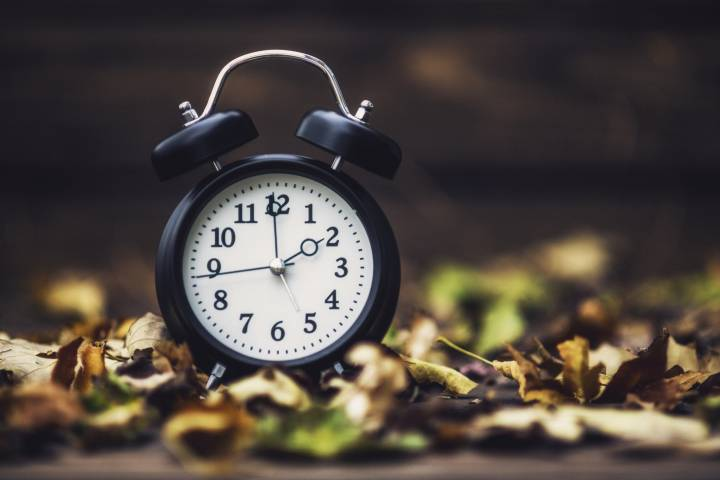
\includegraphics[width=0.2\linewidth]{2018/images/time.jpg}
  \caption{Time}
  \label{fig:time}
\end{figure}

Figure \ref{fig:time} shows a clock. Clocks always denote the passage of time. 
They have the ability to show what the current time is, and how quickly time
is moving compared to our own thoughts. Time is another interesting obstacle in 
this life. It has many different meanings to different people. But it is a 
showing of a passage as it were. A continuous moving section which doesn't stop 
or pause for anyone. It does not move in reverse either. It is constantly moving 
forward.
\section{Sun, Jun 24, 2018}

What determines faith exactly? What determines right and wrong according to a
religion? What determines that the thoughts and teachings passed down from
generation to generation are right and true? Family members scold you for not
following their wishes. Those things they brought you up with. Those things they
expect you to follow no matter what.

It becomes confusing.

More confusing than anything else. Confusing in the fact they won't allow you to
live your own life. They want you to follow in their footsteps without
questioning any of it. There is no room for error. No margin to allow you to
simply be yourself. It is their way or the highway after all.

Personally I don't believe God would intend his children to be brainwashed like
this. To destroy them mentally in such a manner? I don't believe it for a
second. It's a mess. A complete mess that makes people wish they didn't exist.
It sickens me to my stomach, I cannot breathe when I think of such things.
\section{Tue, Jun 26, 2018}

Another day has come to our fair city... or world... or whatever you wish to
call it. Yeah let's just call it whatever the heck we want to call it. Why not?
There's not much going on in the world that can be depended upon these days...is
there? I'm not sure. Perhaps life would come around as it wanted to and we would
all be better because of it. Maybe not. Who's to say exactly what will happen in
this life? No one can know for sure.

\st{
There are times in this life where I just feel like screaming and/or ripping my
hair out! Yeah we usually don't talk about such things. It would be rather
annoying to constantly remind ourselves that we don't enjoy the simple things in
life. That this life is but a terrible dream which we want to wake up from. A
nightmare as it were. Nothing in this life will be wonderful ever. That's not
how any of it works. There are times where life will get in your way, it will
try and make you go down to whatever level it wants you to. There's no way
around it. There's no way through it. Life will eventually come for you... or
the other guy will get you. Either way, someone will get you. That's what this
life is all about. Trying to get the upperhand on someone else? Shame on you!
Shame on me! Shame on the whole world! There doesn't need to be a reason for any
of the contention in this life to be what it is. It is life. It can be wonderful
if we let it. It needs to be wonderful, why can't people see this?

I'll tell you why. They don't want to see it. That's the problem with this life.
They don't want to see all that is wrong with life. They don't want to actually
see what is going on and happening. They don't want to have an understanding or
grasp that which they cannot grasp. They want to remain in a blissful state. A
happy state. A state where nothing can go wrong. Life doesn't work that way
unfortunately. Life is miserable. Life isn't wonderful. Life is crazy at times.
It is terrible!

But who am I to say exactly what this life is or what it will mean to anyone. I
am but a person who lives day to day in the hopes that something good will come
from any of it. All of it. Hopeful? Perhaps. Stupid? Sure why not. Let's call it
that. There needs to be a way for this life to come about better than it ever
was before. Life cannot be taken for granted. It is but a most terrible thought
process upon which we stand. That's right, this life is a terrible thought
process.

Think about that for a moment. How is it a thought process you ask? Well, we are
not currently here. We wish we were here...but we are not. We can't possibly be
here. There's no reason for us to actually realize or think for a moment that we
exist beyond that which we cann't be.

Now that might not make any sense. That could be a most terrible thought process
to be handled upon. We cannot believe that which we cannot focus on. We cannot
understand that which we do not wish to understand.

A person an only declare ignorance for so long until they reach a point in this
life where they are not taken seriously anymore. People have short temper spans
these days. They have a fuse. When that fuse gets lit, they go off immediately.
That's just how the world works.
}

If we knew what was actually going to happen in this life, I doubt we would be
standing around worrying about the things we worry about.\footnote{
Worry is but a construct of the mind. It can be a chemical influence on the
brain much like anxiety. We always tend to worry about that which we have no
control over. Why should we have control over a thing? We shouldn't. Control is
never handeled properly. Why have control over something if you cannot properly
deligate it to the needed places. No one can tell you they will have a complete
understanding of what's going on. There needs to be something which can actually
take control and give order to chaos. Chaos is quite a motivator at times.
}

Well, some might continue to worry. That's human nature isn't it? Yeah, something 
like that. To worry about something that doesn't matter isn't logical. But the 
human race was never logical. I doubt there has even been a 100\% logical 
thinker in this world. If there was? I wouldn't mind meeting them and learning 
from them.

Truth is another interesting concept.\footnote{"When you eliminate the impossible, 
whatever remains, however improbable, must be the truth." Star Trek VI} Where
can we find truth in a world that constantly spews forth hate and lies? Are
there any reasons to believe in such lies? Lies come and go, there are no
reasons to not believe in such things, yet here we are living and thinking about
everything that could go wrong in a lifetime. Here we sit. Hoping someday for
everything to make sense, for everything to come to an end and we will be
sitting there thinking how well we did. Well, I don't think that will ever
happen. This life will come about to an end and we might be sitting there doing
exactly what we are doing now. Waiting for something better to come along.
\section{Wed, Jun 27, 2018}

Headaches. What are you going to do with them? They come, they go, they stick
around and they are evil! Evil I say! What exactly are you supposed to do with a
headache that doesn't leave? It moves around but doesn't leave. Grrr I say, Grrr
to them all!

Whatever the case, there is nothing wrong with thinking. Overthinking can be a
problem, but thinking in general can be good. To think about something is to try
and grasp and understand what is being taught. There's nothing wrong with that.
One has to be able to research and try to understand that which they are
learning. If they do not? There is no purpose in learning and no purpose in
understanding. To think for your own self without relying on other people's
thoughts and wishes is to own your beliefs.

Feelings are something else which can betray you. Feelings can often be
misinterpreted and misrepresented. There are those who would base their faith on
their feelings, but those feelings cannot always be valid. Any kind of feeling
can cause your demise. There is nothing you can do about it. Faith cannot be
based on a fallacy such as feelings. It is not logical.\footnote{
Ah there's that word again, logical. What is logic though? I know I've 
\st{talked} wrote about it before. But that was just a quote now wasn't it?
Yeah, something like that. If someone understands logic, then they are far
better off than I am.
}

To feel okay with yourself is a must. There are days where no one ever fully
feels okay with themselves. They don't grasp the concept of self worth or self
love. It is a sad thought that people have such feelings and thoughts. It occurs
to more people than you would think.

Self acceptance can come. It will come. Yes it might take patience and a lot of
ressaurance, but people are able to come to accepting themselves as they are.
People who press down on them, and try to dictate what is right and wrong in
their lives are not those who should be around you.
\section{Thu, Jun 28, 2018}

Changes come all along the places we will end up. There's nothing left of
anything else long ago the world did end. No one wanted anything else, it would
come crashing down. It is not my fault or determined fate which has the life
upon me. My world will live and continue on if it should only find life. So cast
about your jealous woes of life which easily glide. Nothing else will matter now
a life is but a colliding star.

To grasp and to understand two different things cannot measure within ourselves
a mask is but shrouded long ago into the deepest dark of night. We all be
destroyed long before this life will end. It is but an option yet here we come.
Lost in a moment long ago gone. Oh how gone it all can be long into the darkest
of days and the brightest of nights. We suffer.

Not every aspect of life will make perfect sense. There is nothing more to it
than that which will come to destroy us. Perhaps it comes today, maybe it will
find a way to do its bidding tomorrow. No one has a full clue, no one knows or
understands, grasping all there is at the end of th eday. We are but a simple
vessel seeking and living through this life in the darkest mirror possible. Oh
what a mirror upon which we weep. Lasting but a fleeting moment to bring us down
tot he depths of a great monster. A beast from which there can be no full
escape. To do so would invite that spark, an element of surprise. Maybe not all
at once, but for now it might be a good thing. Something simply wait for you.
That something will find what it wants and needs. Nothing else will come from
it. We are but alone in our thinking.

Now there are days upon more days when none of this will come to any good thing.
It will eventually be our own undoing. Thought this med was supposed to slow my
mind. Maybe it has worn off by now? Who is to say what is going on in this life
at this exact moment. To feel this way, we are but a pain destroyed, reborn and
waiting to come alive all over again.

What a nightmare all of this has become. We are but a person trapped within the
simple brain dynamic. Nothing can ever come good from any of it. This life will
need to come away and be destroyed. So I shall quietly sit here and sip on my
water. It knows what my body needs and that which can be placed aside. Such
nonsense to be held and yet here we are simply waiting for summer to come.

It is cold.

Not like everything else is happening all at tonce, or maybe it actually is.
Such a life barely exists beyond the happy feelings which come from any of it.
We are but a consequence of our own actions. Actions come and go, they tend to
destroy. They tend to create fear and feed upon those things which are right or
wrong. Fear has a tendency to destroy a person deep from within. Not everything
has the ability to survive such an attafck. Oh attacks come and go, they don't
matter why th ey are attacking, only that they are attacking. Nothing has to
wonder at that point. The enevitable will come crashing down someday. Where will
you be when it does come around?
\section{Fri, Jun 29, 2018}

There are some days which come and go as they wish. Nothing is real anymore,
there are so many obstacles in this life, are we alone in our thinking and
thought process as it were?

Whose to say how any of this life or world will form and shape itself as we grow
beyond our own abilities and programming. Do we not have such an internal
programming? Are we not concerned with everything which comes down our own path?
Out of all the many thoughts and ideas out there, one would guess it's more than
a simple aspect of life which we grasp hold of.

Perhaps this is complete nonsense. Maybe it is something else. Either way we
must not be able to think we cannot do something. It isall within our power and
our grasp. But, how far is our reach exactly?

What sphere of influence do we have to deal with? How exactly does all of that
work, how does that happen?

Perhaps there are days which don't matter and won't make a bit of difference in
the long run. We are all but weird creatures swamped within our own mortal coil
or shell. We cannot be allowed to overthink or underthink the possibilities
which will eventually come along our path. Is it in our own destruction to find
that which we cannot find on our own? How does a person even begin to comprehend
such a thought process? Is it not the right timne to wonder and grasp th at
which we cannot hold onto in our lives? Maybe I am at a loss as to the thoughts
within my own mind. An odd cage as it were. Something of naught upon which
everything is founded.\footnote{Feels like I'm quoting movie quotes or something.}

However to live our lives in harmony and to be true to ourselves we must want to
have such a truth made upon us. We have got to be able to find whatever truth
there is to be had and seek after it. It doesn't matter how many people are
following a specific truth, even if it is a small number, that truth's validity
doesn't diminish. It is still truth. To seek after truth is a good thing, a
godly t hing. Truth is an amazing thing to behold.

Wherever truth may be found, if it is good, we must seek after it. Truth and
fact do not always agree with each other. There is truth and then there is
righteous truth. Know the difference.

So, what of it? Who makes the final decision when it comes down to the
possibility nothing matters in this life?

Who is to say exactly what will happen to my family? Not everything is so cut
and dry. Everything comes at a price. Nothing is free as far as anything is
concerned. Are we not simply sheep huddled together for warmth, hoping our
master will come back someday? If so, where does that leave us?

To feel happy. To be happy, in this life we are to try and acknowledge we have a
say in how this life turns out. It is not destiny, it is not some kind of pre
determined thought process. Nothing of that kind of thinking exists.

If we are wrong, then we are wrong.

There comes a time in a person's thought process which we must strive to be
greater than what we currently are. There is nothing wrong with this. Everything
will continue to break down and give way. Why bother with any of it? Whose to
say people won't be together in the life hereafter? Whose to understand and
grasp fully how this life will end? No one has a full grasp of what is going on.
Not even those in higher up places of management.

Long gone are the days where someone said ``Thus Saith The Lord" for we are now
told they, some, were speaking as men and their words are not to be taken as
doctrine, even though they temselves claimed it to be doctrine.

There are so many different things to consider in this life. Doctrine shouldn't
be confusing at all. Why the need to make things so difficult for this life as
it were? There doesn't need to be anything so stupid or selfish from any of it.

This doesn't quite make sense. Are we here for the right reasons or are we
simply here to be puppets, a lab experiment for some God who enjoys watching His
children suffer and wander in unbelief. Hoping they will find and follow Him.
\section{Fri, Jul 6, 2018}

A weekend is here. What more is there to say about it than that? I do not dare
say, for I do not know. It is what it is. Is that not enough thinking for one
day? Perhaps it is. Yes, today is but a day. Another day to try and grasp that
which is meant to be understood and grasped. Something else which is meant to be
looked at, a feat within itself. Nothing else can matter at this point, for it
is but a day. How's that for repetition? Yeah, I thought it was rather annoying
as well.

To be honest, some people tend to repeat themselves. I've been known to do it.
It wasn't right at all. Such thinking can be bad I believe. But that is a
personal belief. To keep thinking the same things over again, is to keep telling
yourself one thing when you know and trust in something completely different.

Is that how this life is meant to work? I do not know.
\section{Thu, Jul 12, 2018}

\lstinputlisting[language=Java]{2018/MathMaxMin.java}

Somedays you just have to take a look at something, anything, be it math even
and see what it does. Maximum values, Minimum values. Values of all kinds. Each
have a story to tell.

Then there are days that you don't want to believe or think about such matters.
But it happens. No matter what, life is always there. It's not going anywhere
for the most part. It'll let you know what's going on.
\section{Fri, Jul 13, 2018}

Ah Friday the 13th. It's a day. It's a thing. One of those dreaded days of the
year which we come across every so often. I wonder if someone has made a
calculated approximation of how often this day actually comes around. That would
be interesting to see actually. I'll have to do some looking into that.

But all I have is this awesome way of checking if a value exists in an array:

\lstinputlisting[language=Java]{2018/CheckArray.java}

Not too shabby if I do say so myself! Now I can't recall where I picked up this
wee little bit of knowledge...somewhere from the great internets I'm sure. I
just don't know where exactly. Oh well. What happens happens and we all have
nothing to worry about if that's the case. I have the code, and that's really
all which matters yes? Maybe. Well as long as it's simply an example piece and
not an actual full blown application...'cause that would be wrong.

But the internet is littered with example java code all over the place. Who's to
say who wrote the original one after it's been passed around for so long?
There's an interesting piece of thought. Who wrote the original piece of code
that we see in examples all over the place?\footnote{
I actually wouldn't mind figuring that bit of history out. I mean...if it's even
possible! I don't think it is. It's like a story that's been told year after
year, decade after decade...passed down from generation to generation. Who's to
say what is \st{real and what is fake anymore} the original real story from the 
beginning.
}
\section{Sun, Jul 15, 2018}

Been working on some things as of late. Nothing too
important mind you. Just some interesting things. There's
a section of the LDS Narrative which isn't in use anymore.
It's called the Journal of Discourses. The LDS Church no
longer confirms these as valid resources. So I started to
compile places where they've been used.

It was quite boring actually. But when the church controls
the narrative, they decide what is used and what isn't used as
can be expected. So yeah, it got boring.
\section{Mon, Jul 16, 2018}

Another weekend is over. A week is just beginning. It is what it is mostly a day
where things happen. Nothing happens because it wants to of course. There is
always a cause and a reaction to an event. This is what life is made for. This
is what life is about. At least I believe that's what it is all about. Who is to
know exactly what life is meant to be?

There are days in this life where we all just want to simply sleep away. There's
nothing wrong with that thinking. However, it must needs be to have some sort of
accurate representation upon the world as a whole. Or upon ones self as a whole.
To be accepted in the world and not of yourself doesn't hold much merrit. Sure
you have the world to thank for your achievements, but if you do not accept
yourself, what have you then? A blank slate. A person who doesn't wish to be
here. That is all there is in life at that point. It  doesn't matter much beyond
anything else.

So here we are. Simply trying to live a life that is worth living. Seeing out
there the things which are meant to be seen. Enjoying everything there is to be
enjoyed without causing harm to ourselves.

It is an adventure at least. Perhaps a misadventure. Either way, we are here and
that's all which matters.

\st{Mistakes happen in life. They really do. But what are you supposed to do
about mistakes then? Do you take them as they are? Do you allow them to run free
in the wild? What of mistakes?}\footnote{\st{What of mistakes indeed. There are so
many thigns in this life which do not make sense. We are here for a purpose
so we are told, yet we do not know all there is to know about any of it. So here
we are simply living life to the best way we can.}}

Perhaps a person can try to understand the reason why they are here. Maybe they
can't. Is there ever a full reason why or why not something happens in life? I
doubt it. Only that we are meant to try and understand to the best of our
ability what we are doing here. If we can understand that, at least that much,
then we are better off then we were when we began.

Reason is hardly ever reasonable. It is but an annoying fly which is in your
house to the point where you do not wish it to be buzzing around you anymore. Or
is it bees that buzz? Oh that's even worse! A buzzing bee flying around your
house bugging you. Yeah, that's the ticket! Such a life upon which we stand, and
still don't have a full understanding of anything of it. We are alive, is that
enough? Perhaps.

Speaking of mistakes. Who's to say who makes the mistakes exactly? Who's to say
what those mistakes are? What makes up a mistake? Is not one person's mistake
another person's treasure?\footnote{What is determined to be a \textit{treasure?} 
There can be so many things classified as treasures these days can't there. Life 
comes along and there are things to be seen and heard. Life has many choices in 
it, it isn't a simple thing to undertake. It is what it is.}

Let us not forget that which is most important a dear to us. There is a time in
life which cannot be shattered upon broken dreams and realities. Life comes at
us once, we have the opportunity to take unto ourselves this life and to see
what is happening an what goes on in our own lives, as well as the lives of
others. It is up to us to determine the best course of action for ourselves.
Were it not so, we wouldn't have the ability to be here. We would be someplace
else. A far off distant shore perhaps, or a place beyond that which we consider
home. Someplace beyond the nebulas of this realm. It is but a dream to some, a
pipe dream to others...this is what life is.

\st{As a youth, I was often fond of playing in the front yard. A man drove by
one day, stopped and asked a question. I answered the man, he had his family in
the car so it was alright to answer such a question right? I do not recall what
the exact question was...just that he asked it and went on his way. My father
saw the exchange and reminded me the importance of not talking to strangers. It
is true I didn't know who the man was, where he was going, where he was coming 
from...I did not know the man at all. An important lesson indeed to be found
among the various memories I have from my years in this life. Years later, I
still don't enjoy talking to people I don't know. Call it being an introvert,
or consider it being something else...whatever the case, it is something I don't
really think about or consider. I try to avoid people as best as possible. Not
the best way to make friends or to gravitate towards people...but it works for 
me, there's no reason to get to know people I don't know or will never wish to
know. But that is just me. There are people out there who can talk to anyone, 
they are able to strike up a conversation without problem. I am not that person.
Not in the slightest, and I am okay with that thought.}

There are things in this life which don't always make sense. I have touched on
this a lot in the past. Perhaps a little bit too much? I do not know, nor can
I say with a full thought process of it all. I do know for a fact that this life
can be a maze if you allow it to be. There is nothing wrong with that, it is
what it is and will be what it will always be. If we are here as a test, under
some kind of sky being then so be it. There is nothing wrong with that. We must
be able to grasp and consider everything which is possible. If we are to take it
upon ourselves to govern ourselves, then we must govern ourselves with accuracy
and be able to understand and grasp that which has been placed in our laps at
the time we are able to do so. \st{It is not above the god given law of self.}
It is not above that which we are capable of. We must govern outselves in times
of need and times of whatever comes our way. We are not immune to the effect of
such matters.

I do not wish to dwell on the negative aspects of life, but it tends to happen
from time to time. It comes and goes as it pleases. There is nothing wrong with
thinking negatively about such matters, but here we are living to the point
where nothing else can take form. We are here. We must accept that fact and we
must move on.

What we remember or don't remember from a past life, or another life as it were
doesn't matter. Why should it matter to us? We are but people living in a huge
gigantic universe. A spec of dust compared to everything else in the world. This
is what life is about. Our nothingness. To understand and grasp that we are
nothing is but the first step in life. There is nothing wrong with that thought.
\section{Tue, July 17, 2018}

There comes a time in life... many times in a life where one simply does not
know where to go or what to do. They do not understand pretty much anything
which is tossed about around them. The person, themselves, can feel quite lost
during these times. There's nothing wrong with such feelings. Teachings of the
past flood their mind, they do not understand or know what is going on. Being
confused about it all hurts. It's one thing to have a belief system, but when
that belief system comes crashing down around you where does that leave you?

To go back to the days where you believed so innocently. There are times when
that would be nice. But they aren't always possible. So many thoughts come and
go in and out of the mind at times. It can be overwhelming, and even then that's
just being nice.

So, what does one do about it? Do they keep marching on as if nothing has taken
place? Do they confront the issue at hand? What are they to do about any of it?
So many questions with so many uncertainties and unanswered everything. Talk
about a rollercoaster. I wish at times I had never embarked on this journey, but
now I know what I know. There's no turning back.

Where is the truth? Where is the lie? Where is the falsehood? So many questions
and so many different opinions on matters. It is but a differing of opinions at
times. Sometimes it is better other times it is worse. Either way, unless you
come up with some kind of equation to figure out what is truth and what is
false, you will fail eventually.


\begin{table}[h!]
\centering
\begin{tabular}{|c|c|c|c|}
\hline
a     & b     & a (AND) b      & a (OR) b    \\ \hline
false & false & false          & false       \\ \hline
false & true  & false          & true        \\ \hline
true  & false & false          & true        \\ \hline
true  & true  & true           & true        \\ \hline
\end{tabular}
\caption{TRUE/FALSE Examination}
\label{table:1}
\end{table}

Math and Science are fact. They cannot be destroyed. They can however be proven
wrong but another truth will fill its place, using either Math or Science. There
are truths in this world that cannot be altered. They are concrete, no matter
how much you try you cannot change certain things. They are laws which must be
lived by and abided by in the universe there is no contradicting them.

People have tried to contradict certain truths but have found it difficult to do
so. They eventually have to come to the truth themselves and realize there is
nothing but truth in the thing they have been seeking. They must accept that as
fact and cannot turn from it.
\section{Wed, Jul 18, 2018}

Today is but a day, tomorrow is another day which will eventually turn into
dust. Nothing will ever last. It all goes downhill and gets destroyed. There is
nothing wrong with such a thought for that is how the universe will continue to
spin and go around in circles. Yet it is today.\footnote{
We can see at this point in the trials of the author, they are starting to lose
their mind. They cannot confirm or deny this of course, but their words tend to
continue to loop around that which they no longer comprehend. Is it actually a
life story or is it a work of art, a work of fiction.
}

I would like to think for a moment that this life exists for a reason. Beyond
anything that religious beliefs have brought about and taught. It is here for a
reason, a good reason? Maybe. Some kind of reason to be sure of. If that is not
the case then this life is lived in vain and everything else which belongs to it
can and must be destroyed along with everything else.
\section{Thu, Jul 19, 2018}

Life can be frustrating at times. There's no way around it. You will have
difficulties in this life. That's all there is to it. That's the most simple
fact of it all. You can't escape it, you can't run from it. It's not that you'll
be doomed or anything, just that life will make its twist and turns and there's
nothing you are able to do about it. That's fine though. it's life. Eventually
things get figured out right? One would hope so.

Watched a movie last night. It was about a guy who could time travel, and time
travel he did. By the end of the movie, he decided that life wasn't about time
traveling but the ability to realize that each day is precious and to live like
you have gone into the past to make changes. It was an inspiring film, quite a
moment to be had for sure.

I oft wonder at times what it would be like to change something in my own life.
There are some things I wish I could change, but the more I look at them I don't
think I would change them. Those moments are what made me the person I am today.
Changing them would in effect change me. I suppose if I were to be able to
change something, I wouldn't want to have a knowledge of both the former me and
the new me. I suspsect that would become confusing.

Think about it for a moment. You have this knowledge of a former you, things and
events didn't happen in this new timeline of events since you changed them. What
would that do to a person's psychie? Since timetravel isn't possible, I don't
think we would have such an answer. But it is something interesting to think
about.

Feelings that come along in this life alone are confusing. They tend to cause so
much inner struggle. Feelings, emotions, whatever you want to call them. They
serve a purpose I suppose, but somedays I wonder if it would be better if
\st{we} I didn't even experience such things. But \st{we} I must deal with these 
thoughts and feelings, some come from damaged pasts, depression, anxiety and 
whatnot. Either way, here \st{we} I am \st{are} doing the best \st{we} I can do 
without looking back. Never look back. It will destroy you.
\section{Fri, Jul 20, 2018}

Happy day, it's Friday! I mean honestly, what's better than a Friday? Perhaps a
Saturday, fine I'll give you that. But today is Friday and that's good enough
for me. I enjoy a good Friday. Not to be confused with Good Friday, that's an
actual day. But just a Friday that's the end of the week signaling the weekend.
Yeah something like that. Yes indeedy!

I remember being in a class once, where the teacher had us write down our
thoughts and feelings about certain topics. Near the end of th quarter, he said
if we aren't personalizing it to ourselves, we aren't putting enough time and
effort into the writing. At that point, I hadn't done much of anything so I
started writing sentences with more I's in them. Making it more about me than
general thoughts. It was a good experience. I find myself slipping in and out of
such writing these days, sometimes I write more about me other times I write
more genrally. It's a toss up. But I need to get more into the habit of
personalizing things more. That would be a good thing.

There was another time I was sitting in class, the teacher had quoted from a
paper he handed out to everyone. It talked about being restricted, held captive,
if you couldn't move and were bound were you really bound? Everyone in the class
agreed that you were. But then the teacher asked if anyone thought opposite of
what it said. My hand went up. Apparently I was the only one in the class that
was thinking that morning? I'm not sure.

I argued the point that even though they might bind a person, physically
restricting their movements etc, they will still have the ability to think for
themselves. They cannot take that freedom away from them for they cannot know
their thoughts. Mind control is a thing, it can happen, but I suppose it all
depends on a person's willpower. If they have the ability to deny thoughts
thrown at them and can have the ability to be strong through it they cannot be
bound and cannot be broken.

It's an interesting thought to this day actually. There are so many types of
oppression\footnote{
oppression

\textit{noun}

1. Prolonged cruel or unjust treatment or control.

2. The state of being subject to unjust treatment or control.

3. Mental pressure or distress.
} in the world. A person can be dragged through the mental gymnastics of a cult,
or religion\footnote{Is there a differenced between the two?} and can be torn
left and right beyond anything which they are able to \st{feel} withstand it 
would seem. It's a cruel thing to force someone to go through.

I wish I had that exact quote I mentioned above, it would be a nice addition to
today's thought process. But I cannot find it. Maybe I'll find something simliar
to it? I don't know. Onward I search.
\section{Sun, Jul 22, 2018}

So many confusing aspects of life come about because people don't grasp their own
history. When people do try and attempt to understand that history, they are called
unto repentence because it's showing negative light upon the church. A church which
doesn't want its history to be made and known public doesn't have a leg to stand on.

\st{So many confusing...} There are really things out there which don't make sense.
It would be nice if they actually did make sense for once. But they do not and so we
are left with our own thoughts and processes upon which we are meant to try and
understand that which we cannot. Some would tell you to simply wait until things get
better, until a time when we are able to understand all of it, we are meant to have
faith and act accordingly.

What if I don't want to waste my time?

It never ceases to amaze me, when something bad happens in a person's life they think
it's a sign from God. That there's some reason they're having this difficulty and
it's a blessing that they are going through such an experience.

That's not always the case.

Sometimes bad things just ... happen. Bad things happen to good people, they happen
to bad people. Bad things really just happen. There's no reason to expect it's a sign
from God or that God is putting you through a trial for a specific reason. I wish
people would accept and understand that better. But they don't.
\section{Mon, Jul 23, 2018}

Cars on the freeway. That's what life feels like at times. Just a bunch of cars on a
freeway. There's nothing wrong with cars on a freeway mind you. Until they end up
getting into an accident, or backing up the freeway so you cannot move forward.
Obviously you can't go backwards either. But you sure as hell can't move forward.
That's what this life is about. Always  moving forward, sometimes you are stuck in a
section for a while. That would be where the freeway is stopped. But other times you
are inching forward towards whatever goal you have. It's not always a fast
progression either. When the freeway is moving fast, that's a good sign.

Times change and so do people. People have the ability to make changes in their
lives. There's nothing wrong with that. Change can and will come at the decision of
the person needing the change. I don't doubt God works in this way. If we are to have
joy in this life and something isn't right, we need to make a change. That change can
come within, we do not have to wait on revelation from God for that change to take
place. Goes back to not being commanded in all things.\footnote{D\&C 58:26 For behold, 
it is not meet that I should command in all things; for he that is compelled in all 
things, the same is a slothful and not a wise servant; wherefore he receiveth no 
reward.}

So, if we are to think for ourselves and not expect God to fix everything in our
lives. Then we are able to do that which we must do to make our lives better. Why
don't people tend to see this? They have the charge to do it. It's up to them to make
their life better instead of complain that God hasn't come down and changed things
for them. God won't interfere like that. It's not in the program for Him to
interfere. Why don't people grasp that? It's a most basic principle.

I've often wondered what it would be like to write a letter to my parents regarding
my current religious beliefs. It wouldn't be an easy letter to write. I suppose these
things are never easy to write, are they. Well that's the delima I find myself in. Do
I tell my parents my beliefs? Do I shatter their world? What would that letter even
look like?

My wife has told me to wait till they die. Which can be harsh, I'm not gonna lie. But
if it prevents heartbreak in this life, why not. They don't need to know my beliefs I
guess, I mean they already have thoughts I don't believe anymore. But we don't really
talk about it, and why should we? It only causes contention and strife.

Being told that contention is of the devil\footnote{
3 Nephi 11:29 For verily, verily I say unto you, he that hath the spirit of 
contention is not of me, but is of the devil, who is the father of contention, 
and he stirreth up the hearts of men to contend with anger, one with another.
} for so many years, I tend to avoid contention. I hate it, it's not producitve no 
matter who's behind any of it.

My parents did tell me to write my own book regarding the church, but I'm not sure if
they understand the kind of book I want to write. The truth of things is what is most
important. Be it spiritual truth, religious truth, or personal truth. The truth must
hold strong and will always be dear to my heart.
\section{Tue, Jul 24, 2018}

Tuesday, what on earth do you say about a Tuesday exactly? I mean, it's a day. It's
the second day of the week granted, but it's just another day. There's not much to be
said about today. Sure it's a Utah holiday, whatever. That's nothing special, not
when you have to work on the holiday. So there's that. Forget the holiday aspect of
today. Nope, no reason to deal with that.

What else is there about today that makes it special?

Haven't a clue.

However, I did find this happy image. Sure it's photoshopped, but it's still fun:

\begin{figure}[h!]
  \centering
  
\includegraphics[width=0.5\linewidth]{2018/images/truth.jpg}
  \caption{Truth}
  \label{fig:truth}
\end{figure}

We have been charged to find the truth in all things. If it contains not the truth
then it should be \st{destroyed}\footnote{Destroyed might be the wrong word here, 
dismissed maybe would be better?}. It's really that simple, is it not? I would think 
it to be.
\section{Wed, Jul 25, 2018}

\centerline{But what if you're wrong?}

That's a common question to be asked to religious folks isn't it? So many damn
confusing things in life and people still don't grasp the question, what if they're
wrong. What is there to be wrong about? Plenty. The nature of God, who He is, how
things came to be in this life etc. So many possible outcomes to the answer as well.
The most devout will say they aren't wrong, they are in the right no matter what.

Some will tell you, well if I'm wrong then I'll be okay still. What hurts to give
that extra effort? What could hurt if they are wrong? They're still living up to what
they believe is right, so it's good right?

Not all those who profess to know Christ will enter thte kingdom of heaven, it's
stated in the bible that's the case.

\begin{displayquote}
Not every one that saith unto me, Lord, Lord, shall enter into the kingdom of heaven;
but he that doeth the will of my Father which is in heaven.\footnote{Matthew 7:21}
\end{displayquote}

It's right there, black and white.

Another thing to consider, why worry about another person's salvation if you do not
know the status of your own salvation? Should one not be more concerned with their
own outcome before trying to fix another individual? Are we not told to remove the
beam out of our own eye before \st{criticizing someone else} casting the mote out of 
our brother's eye?\footnote{Matthew 7:5}

I dare think some people forget that part of the gospels, they're so caught up in
thinking everyone else is false that they cannot see the beam in their own eye to
even begin to see clearly.
\section{Thu, Jul 26, 2018}

Today is but a day. Tomorrow is but another day. We are living in the here and now
and that is all which  matters. There is no time like the present, that's a saying
which has been said here and there. If you do not look forward to that which you are
given today, there is no hope for tomorrow. All things which might have been said of
people in the past, I do not know if they have or not. If they haven't, then they
should have been said.

This life is here for us to enjoy it. To be understanding of anything which comes
into our own minds and heart as truth. We are to seek out the truth and understand as
best as we can the teachings from it. There is nothing wrong with that thought.
Knowledge is a good thing, it is God given and it is here for us to grasp and take
with us on this journey throughout life.
\section{Fri, Jul 27, 2018}

The weekend is here, well it's coming. Today is Friday. The weekend isn't fully here
yet. But it is on its way and that is good enough for me to handle. So here we are at
the final stretches of the week. Some things have been learned this week. Some to
make one angry, upset, and a whole range of other emotions. But there are other
things which do not cause such grief. Happiness tends to come around in different
ways, and that is good.

To be happy is not always a thing to be found in this life. There are so many
opportunities to feel any emotion during a given week. So many places to go and find
and see the many different aspects of life. Yet if a person isn't to be found holding
onto traditions they once grew up with as a child, they are frowned upon. I have
found that to be the case many times in my life.
\section{Sun, Jul 29, 2018}

Why are so many things annoying in life? There should be something done about the
annoying things. I'm not sure what should be done about it all? But well, soemthing.
Anything would be nice. Yes, that would be perfect. Yet here we are simply having to
accept the annoying things which go on and there's nothing we are able to do about
any of it.

So what then? What happens next? Are we meant to just sit here and allow things to
happen? We have the ability to attempt to stop things, this is true. But how many
people actually step up and try to stop it? Any of it?
\section{Mon, Jul 30, 2018}

There is in this life, the thinking that a person can get away with anything. It is
not the correct thinking on anything, but it is a thought some people have. To say
anyone can get away with anything is a falsehood. The law will always catch up with
that person. This will always be the case. If for some reason the law does not catch
up with them in this life, the eternal law and judgement will catch up with them in
the life to come. So yes, the law will always catch up with them.


\section{August 1, 2018}

A new month. New experiences to be had. A life worth living? Perhaps. A life worth
dying for? Well, everone dies eventually right? yeah, something like that. Either
way, it is a life. Is that too much to ask for? Is that too much to say about it all?
I do not know. It will always be this way. Either you live or you die. There is no
other option.

Some would think this life is full of happy places and everything else. It is not
always the case. There are always issues which come up during this life. There are so
many things which happen and which people don't have control over. They look towards
a God or Gods and hope for the best. Some claim to know these Gods are looking out
for them and will help them no matter what.
\section{Thu, Aug 2, 2018}

Got a book yesterday in the mail. The journals of William Clayton, Joseph Smith's
personal secretary. It's an interesting read for sure. I'm excited to have it, I
already began reading through the Nauvoo period, very interesting book.

\begin{figure}[h!]
  \centering
  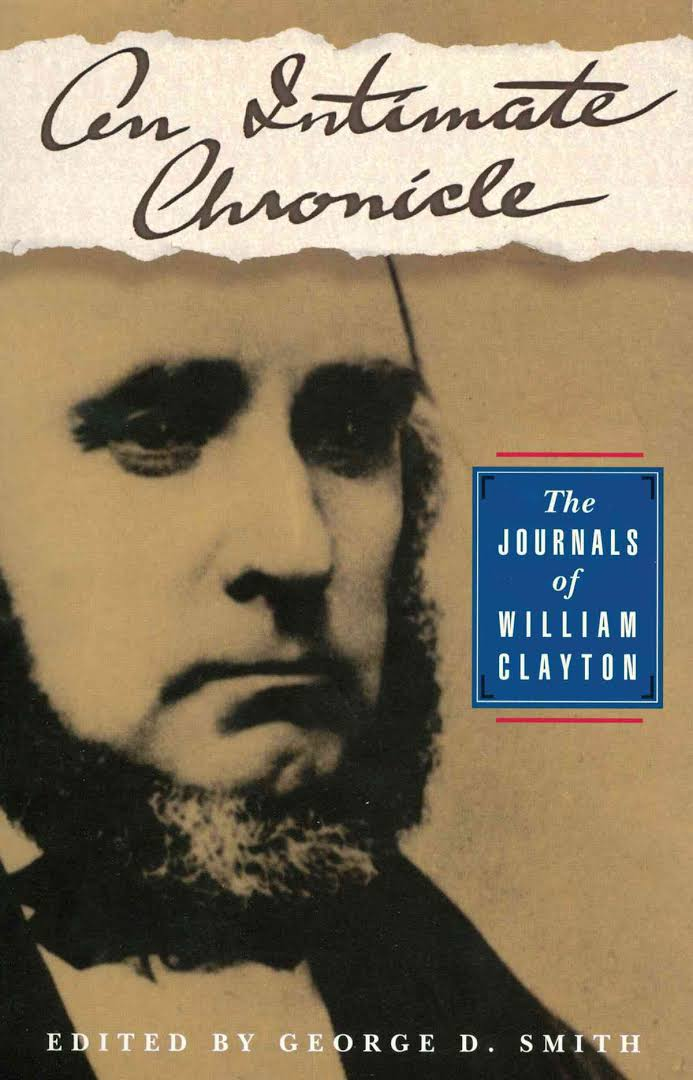
\includegraphics[width=0.5\linewidth]{2018/images/clayton.jpg}
  \caption{An Intimate Chronicle: The Journals of William Clayton}
  \label{fig:clayton}
\end{figure}

It's another day, waiting for bills to go through is not the easiest thing in the
world. We live in a world where transactions can occur instantly. Yet when a person
pays for a bill, it takes forever it seems to go through. What's up with that? I
don't get it. I don't understand any of it. Such an odd weird life to be living in a
times. We have come so far in advancements in technology, and yet here we are waiting
for something to go through. So very very odd.

Oh well, it is life as it would seem to be...I guess. Whatever the case, here we are
just trying to live another day and get by. There's nothing wrong with any of that,
is there? No, I didn't think there would be. I mean, let's face it. Life comes and
goes long after we are gone. We will always be remembered in a place where we were
the most happy, the most plesent of thoughts. There is no reason to think otherwise.
Is that not what people wish to remember about people? The good memories, the good
thoughts upon which they are able to exist? Yes, something along those lines for
sure.

I fear at times, I do not have the adequate knowledge or thought process as those of
old who have gone on before. But I cannot allow it to simply be erased. Whatever I
was in this life is what I was. Whatever I will become in this life, is what I will
become. I cannot change the past. I can only look forward to the future with a
brightness of hope.
\section{Sun, Aug 5, 2018}

Tis Sunday. There's nothing wrong with it being a Sunday mind you. But it is Sunday
and that is okay with me. I think. Maybe. Who's to say if it's okay or not? Today is
but a day of rest, and here we are resting from our labours. That way we are able to
continue onward tomorrow and see all there is to see out in the world. Maybe if we
are lucky, we can see things which are meant to be seen, and that which is meant to
be seen we can see. Trust me, it made sense a second ago.

Been reading lately in the journals of one William Clayton. Came across this unique
piece of history:

\begin{figure}[h!]
  \centering
  \includegraphics[width=0.5\linewidth]{2018/images/clayton2.jpg}
  \caption{An Intimate Chronicle: The Journals of William Clayton, p. 120}
  \label{fig:clayton2}
\end{figure}

Take it as you will.
\section{Mon, Aug 6, 2018}

There seems to be something in the air as of late. I'm not certain what it is or how
it got here. All I know is it's here. There should be something exciting to this
life, but there isn't. It's becoming rather bland. Perhaps I'm just getting
comfortable to it all? I'm not sure. There should be an explaination for it all, but
there isn't. There hardly ever is anymore. Any kind of explaination would be of
benefit, and yet here we are. Sitting, thinking, wondering about things that probably
shouldn't be wondered about.

Have you ever waited for baloons to die? It can be an annoying thought process, and
annoying thing to watch and something obviously annoying to just have happen. They
were full of life once, now they just hang around waiting to have nothing within
them. It's a lot like life if you think about it. People come about and are full of
all this energy, then they evenaully fizzle and fade away without anything else to
sustain them. No matter how into something they were at some point in life, it all
fades away.

I suppose if life didn't ever fizzle, we wouldn't have a problem. There wouldn't be
some kind of issue as it were.\footnote{I guess it all comes down to hopeful
thinking, that's really all it is.}

There is a phrase, which seems to have become a motto as it were. Which is sad, the
phrase:

\begin{displayquote}
My shoes are too tight. But it doesn't matter, because I have forgotten how to 
dance.\footnote{Londo, ``War Prayer", Babylon 5}
\end{displayquote}

The analysis is simple, a person puts constraints on themselves, the shoes, during a
lifetime, and they cannot enjoy life anymore, thus forgetting how to dance. \st{To 
live a life and then to realize it was all for nothing is not an easy thing to
process at times.} There is in this life, a time for everything.\footnote{
Ecclesiastes 3:1-8} Each moment has a purpose, each moment has a time upon which it 
is able to breathe and explore this life which is around us.

If we didn't have the ability to search out and explore such a life, where would we
end up exactly? To be constricted in ones own beliefs, cannot be a safe place to end
up, can it? Everyone needs a safe place in which they are able to be calm. The need
to be able to be safe and have a place to relax is what is needed most.

Memory recollection can be a tricky topic at times. Some people can have the ability
to remember things in perfect detail, while others have issues recalling that which
should be memerable to them. I wonder if it is by design of the human brain that this
is the cause. Is it possible we are not meant to recall things clearly like it
happened yesterday? At which point in our lives does our memory completely falter and
we cannot have the ability to figure out the truth from it all?
\section{Tue, Aug 7, 2018}

\centerline{Part of me wonders why I am sad.}

Even when I was at my strongest, and I was doing everything I could for church and
state, I wasn't happy. I was depressed, sad, down. There wasn't anything that could
``fix" the situation I was in. I have found as time moved on, I haven't ever stepped
out of that place in life. Here I am just living day to day wondering when something
will get better.

Will it ever get better? I've been told by some that it will. I have taken the steps
they have told me to take, and it hasn't done much for anything. I am still the same
person I was over a decade ago. So, where does that leave me? Where do I go from this
point in life and where will I end up?

\chapter{Journal Entries 2019}
\epigraph{But a day to be found in, we need to be lost.}{\textit{Kyle Eggleston}}
\chapter{January 2019}
\section{Mon, Oct 1, 2018}

Today is just another day I suppose. I mean what are you supposed to do
with such things? Not sure. Whatever the case, here we are waiting for
the day to be it.

Monday is always the start of the new work week. It can be a good thing
for sure.

\section{Sun, Sep 2, 2018}

I feel like screaming. Is that an okay thing to do today? I sure hope so, because
well here I am ready to scream. So many thoughts are occurring right now and I'm not
sure where they are going to go or how they will end up. There needs to be a way to
have something done because of it all. Yet I do not know how to go about it. So, I
will sit here and wait for something to happen. Is that wrong? I do not know.

Waiting can be a bad thing, if I wait for something to happen it might never happen
at all. That would be a case of a bad thing. However, if I take the initative and
step forward and make a move? Something could happen. That could possibly be a good
thing right? One would hope so. It could also turn out to be a bad thing.

I think either way I think about it or do something I'm kinda messed up. So there's
that. Oh well, life will find a way to overcome whatever there is to overcome. I can
be content with that thought. Well I think I can be content with that thought. Who
knows.

There are some things that shouldn't be asked of people, of any age. But I suppose
that's what sets me apart from the church. They don't need to pry. They don't need to
get deep into any of it. Leave it at a light simple thing and let it go. What the
hell.

\section{Wed, Oct 3, 2018}

Wednesday, what is there to say about you exactly? I mean, here we are, it's the middle
of the week and what do we have to show for it? Who's to say what will happen when every
other thing in the world goes kapoof?\footnote{Is that even a word? I doubt it, but I
like it!} Then we come to other things that occur in the day. What are those things?
Well, people go to work. People exist. People do whatever they need to do in order
to survive. Is that not the case? Is that not what people do day in and day out? Survive
to another day? Yeah, something like that.

\section{Thu, Oct 4, 2018}

General Conference is coming up. That can be a good thing. I wonder what they'll
announce at it. Is that wrong? I mean people keep saying that President Nelson is all
about revelation, a a rush of revelation, and a snowflake in a snowstorm kind of
thing. If those things are to be believed, then supposedly there should be some kind
of revelation at this next General Conference. However, the types of revelation that
have been revealed have been more of a business standpoint, nothing really spiritual
as of yet...so um yeah, that's where we sit at the moment.

\section{Fri, Jul 6, 2018}

A weekend is here. What more is there to say about it than that? I do not dare
say, for I do not know. It is what it is. Is that not enough thinking for one
day? Perhaps it is. Yes, today is but a day. Another day to try and grasp that
which is meant to be understood and grasped. Something else which is meant to be
looked at, a feat within itself. Nothing else can matter at this point, for it
is but a day. How's that for repetition? Yeah, I thought it was rather annoying
as well.

To be honest, some people tend to repeat themselves. I've been known to do it.
It wasn't right at all. Such thinking can be bad I believe. But that is a
personal belief. To keep thinking the same things over again, is to keep telling
yourself one thing when you know and trust in something completely different.

Is that how this life is meant to work? I do not know.

So many people have questions in this life. Not all questions can be answered by
a simple flick of the switch. Not every question can be answered, period. There
are questions which people have, valid questions. They are looking for answers
to those questions. When they ask their questions, they desire answers. Those
answers do not come. They become frustrated. It's a valid response. If you're
constantly told not to worry about a thing, and to simply let it go. That's
where the dangers rise up. People will seek out their answers. Sometimes they
will leave a place to go and find them. That is how life is.

\section{Wed, Sep 12, 2018}

\begin{figure}[h!]
  \centering
  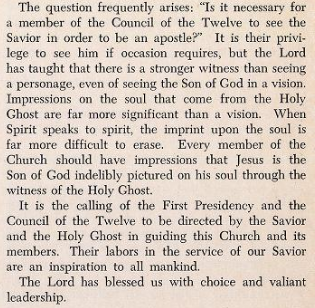
\includegraphics[width=.5\linewidth]{2018/images/apostle.png}
  \caption{Apostles Don't Need To See Christ}
  \label{fig:apostle}
\end{figure}

That quote is from the Improvement Era, Nov 1966, Page 979.

There's an interesting quote if you ask me. They're called as special witnesses of
Christ, but that appears to be in name only these days. In the old world, and in the
americas when Christ visited they were actual witnesses of Christ. For they saw and
talked and walked with Him. Nowadays? Not so much.

Makes one pause and wonder at times. If the church is actually being led by Jesus
Christ himself or just fuzzy warm thoughts and impressions that come to their mind?
They claim it to be revelation, but what exactly is revelation? I mean we have the
passage in the D\&C about it.

\begin{displayquote}
Yea, behold, I will tell you in your mind and in your heart, by the Holy Ghost, 
which shall come upon you and which shall dwell in your heart.

Now, behold, this is the spirit of revelation; behold, this is the spirit by which 
Moses brought the children of Israel through the Red Sea on dry ground.\footnote{
D\&C 8:2-3
}
\end{displayquote}

So, the Holy Ghost speaks to you through your mind and your heart. That's an
interesting thought process. The mind and heart are often at odds with each other,
well from personal experience. So when they are in harmony it is of God and they are
helping to channel revelation to you? Interesting thought for sure.

\subsection{11:12 AM}

Ever have a day where you think you have something figured out, but in reality you
don't even have a clue? Yeah, today feels like one of those days. It's okay to not
have a clue I suppose, I mean it's just what it is right? Yeah, something like that.
Today is just a day and there's nothing that can be done about it.

\section{Wed, Nov 14, 2018}

There comes a day when life is just life. It doesn't always happen that way.
Sometimes we are simply just living here. There needs to be a reason for it. Reasons
must come and go from time to time...that's okay to try to grasp. It's not always an
easy explaination.
\section{Sat, Sep 15, 2018}

Today is another day. That's all there is to it. The inward feelings and thoughts
which come across, they aren't the easiest or best thoughts ever. So here we sit
waiting for something better to come along. Will anything better ever come along? I
do not know. It would be nice for something nice to be able to sit and simply wait
for it to happen. Yet, here I am still waiting for closure. What is it I'm waiting
closure on? Well, that's a long story. Maybe I will say why someday, but now? No. It
can't happen and it won't happen anytime soon. So that's all there is to it.

\begin{figure}[h!]
  \centering
  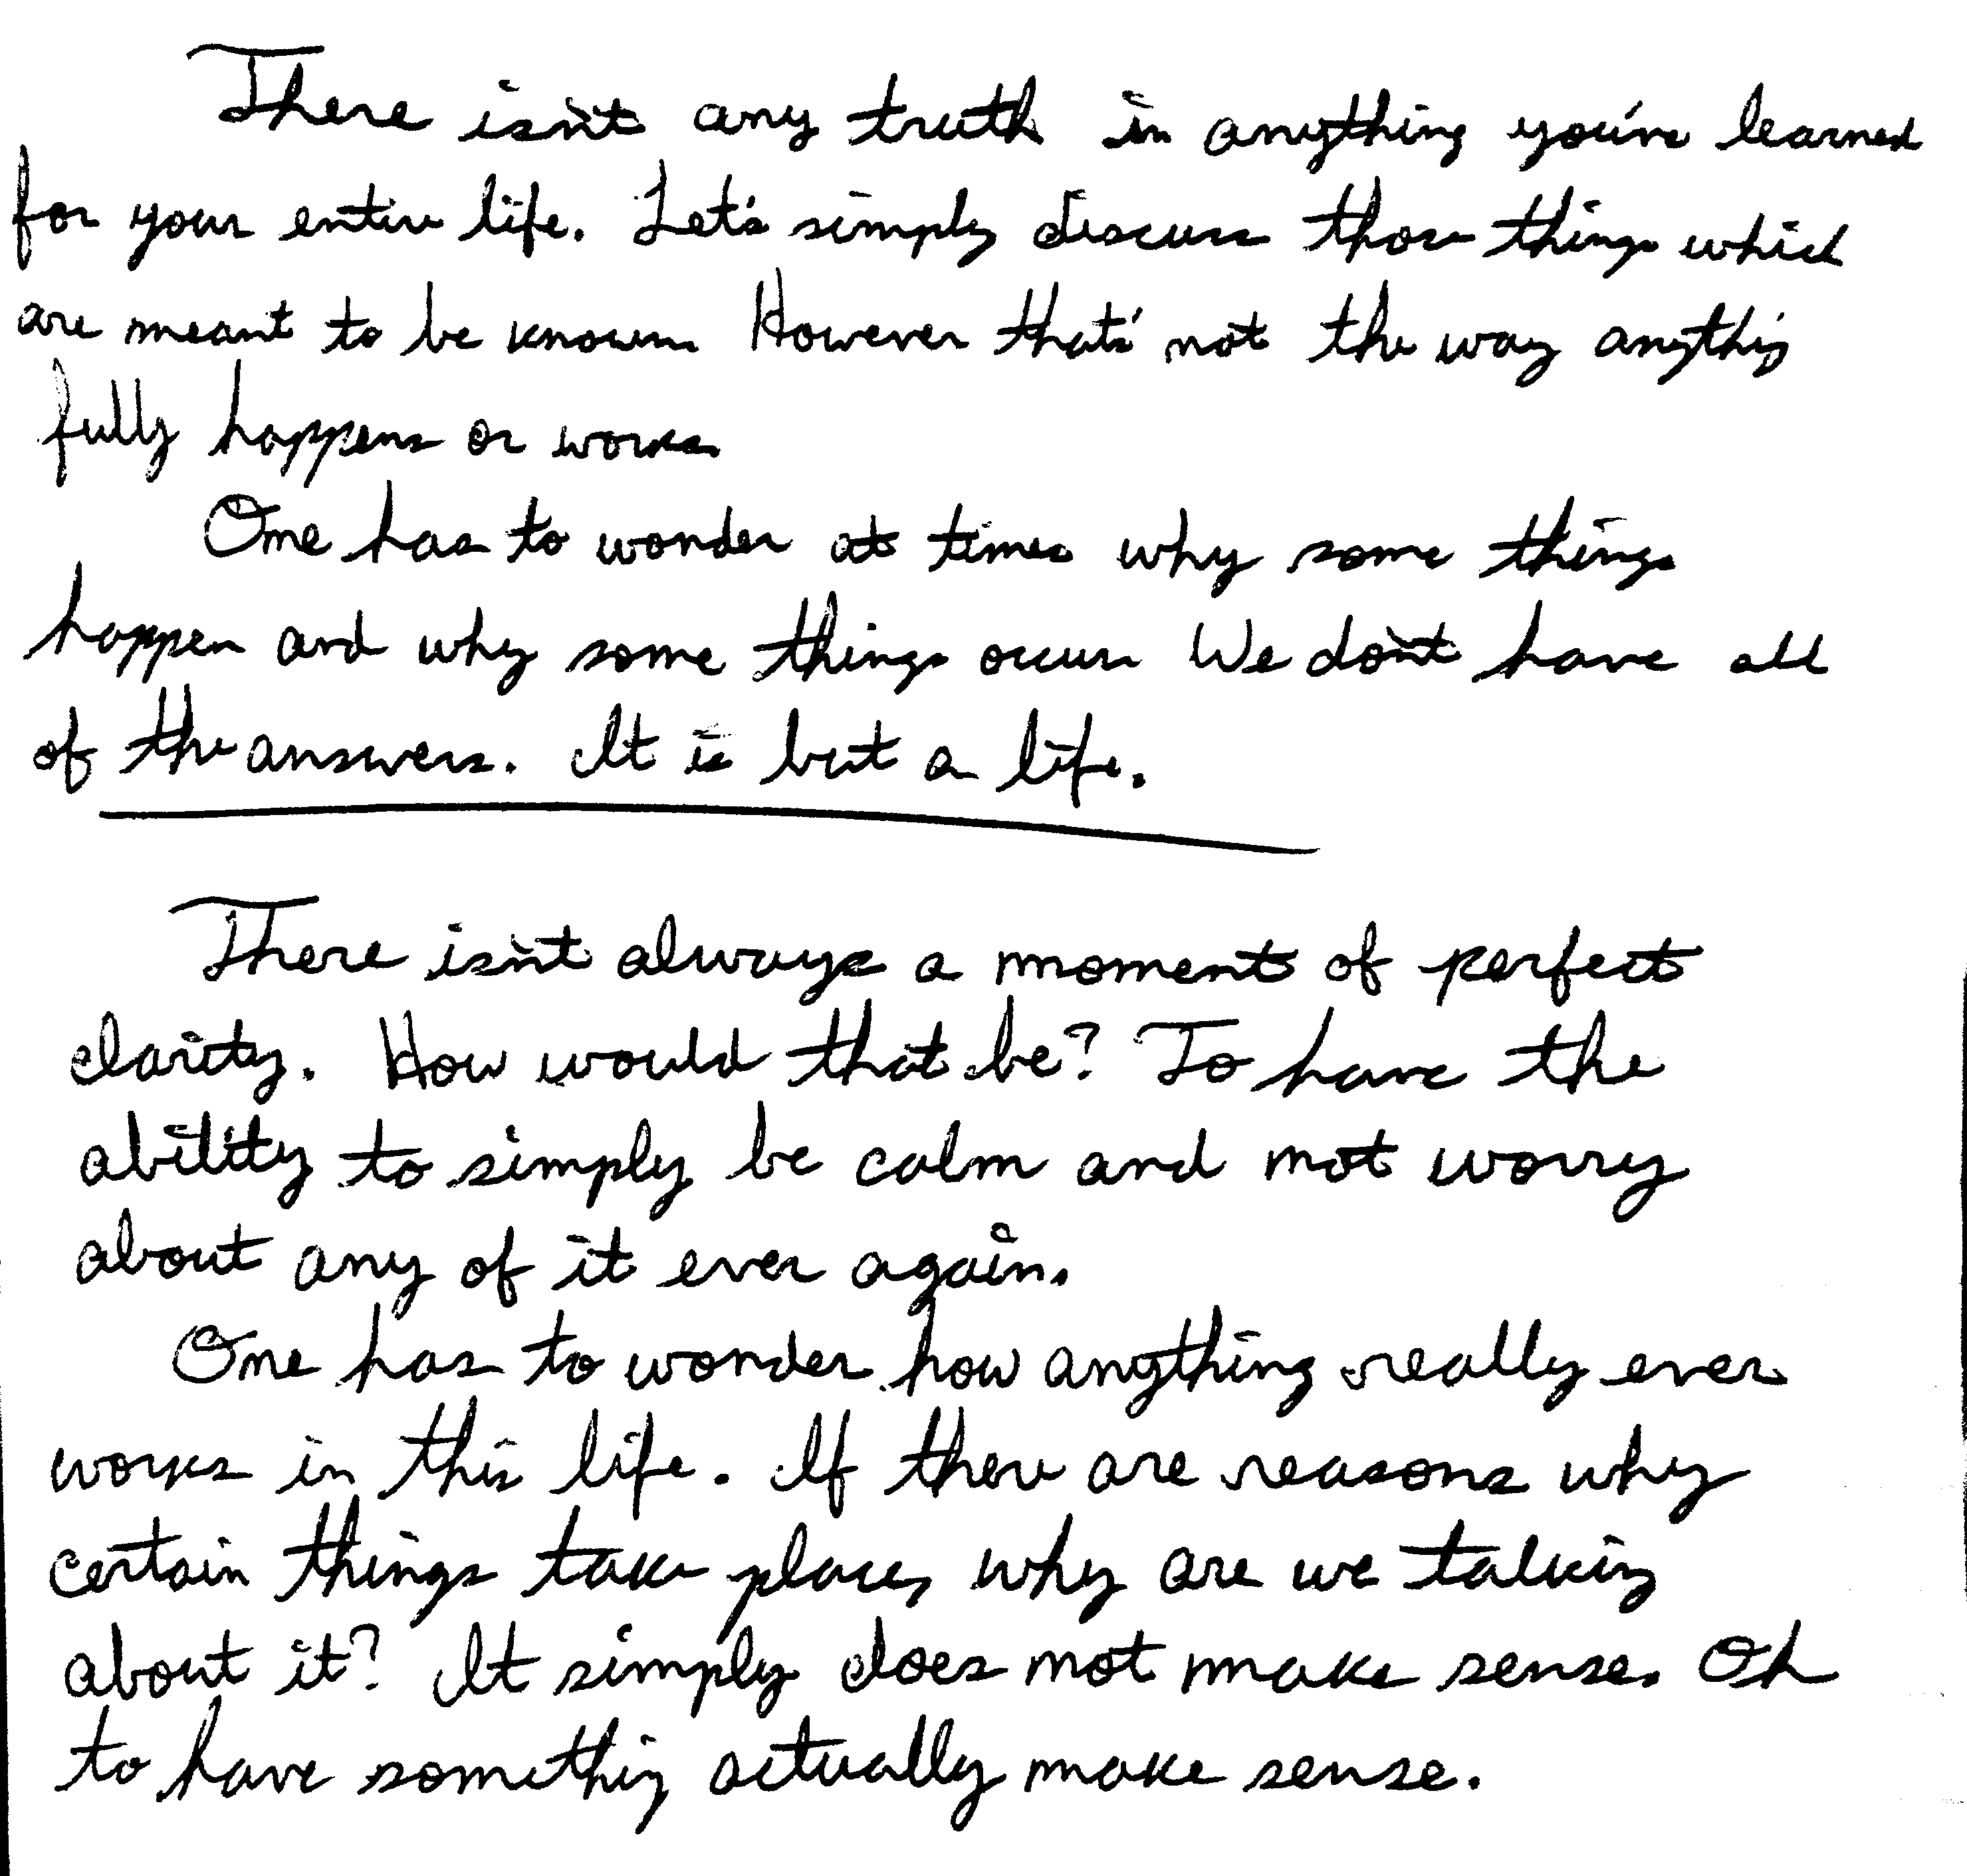
\includegraphics[width=.5\linewidth]{2018/images/handwriting.jpg}
  \caption{Handwriting}
  \label{fig:handwriting}
\end{figure}

Writing things down has a way of calming you. Be it handwriting, or electronically.
Either way? I feel handwriting has the ability to help out the most. When you can sit
down and write \st{some} experiences out on paper? It's a great feeling. It feels
right and has a way of calming you down. Talk about a breath of relief.

There comes a time in a person's life when all they want to do is sleep. They want to
forget everything about the rest of htis life and simply desire to fall asleep never
to wake up again. It is only a natural part of life is it not? Death is part of life.
There has never been any teachings contratry to that notion. It is the next
eveolutionary process in the steps of man.

So, why can't a person select the time of their own choosing? I mean, isn't it enough
to say ``hey, I'm done with this life. I'd like to go home now." Is that such a bad
thing? I do not know.

\begin{figure}[h!]
  \centering
  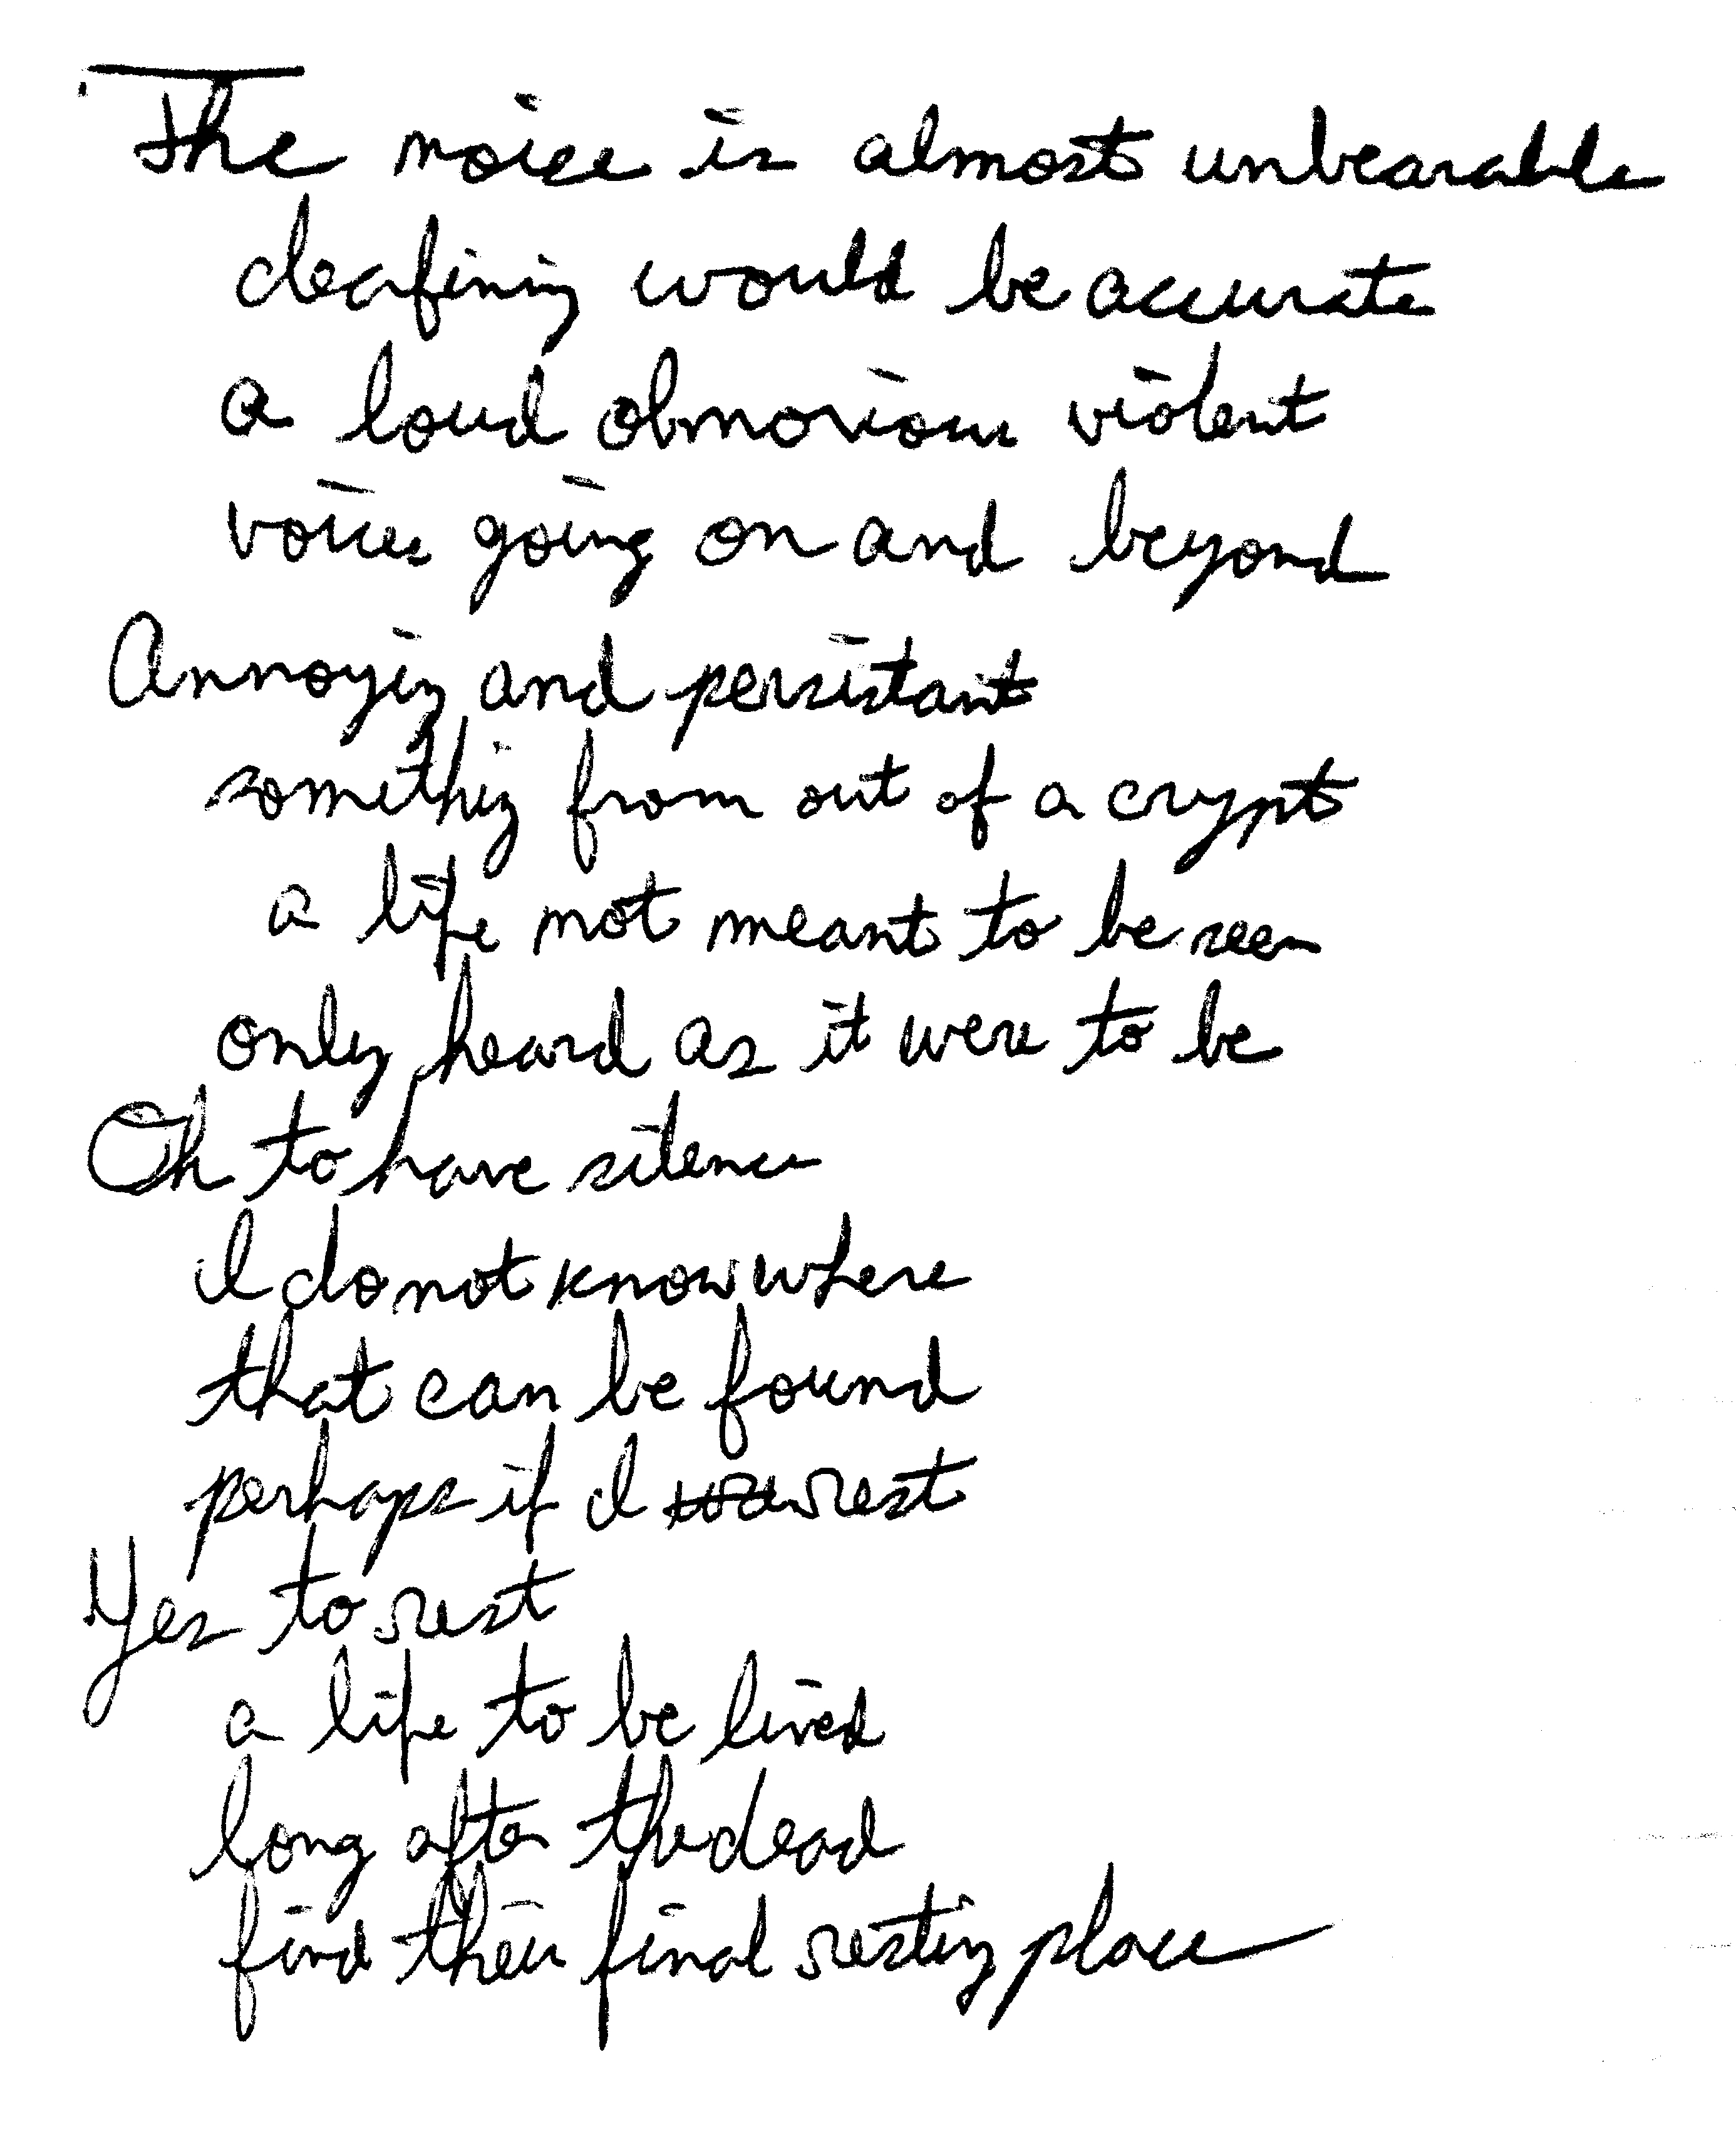
\includegraphics[width=.5\linewidth]{2018/images/rest.jpg}
  \caption{To Rest}
  \label{fig:rest}
\end{figure}

Perhaps it is a fixed point in time that we are unable to change. So many options and
changes come through this life, and here we are hoping one of them will be good
enough of a change for us ourselves. What if that's not the case at all? What if such
a change would have to come from a different source? We have agency, as it were, so
why cannot we enable such a change to be made and binding?

\section{Wed, Jan 23, 2019}

Lawrence E. Corbridge stated the following:

\begin{displayquote}
\begin{enumerate}
\item Is there a God who is our Father?
\item Is Jesus Christ the Son of God, the Savior of the world?
\item Was Joseph Smith a prophet?
\item Is The Church of Jesus Christ of Latter-day Saints the kingdom of God on the 
earth?
\end{enumerate}

If you answer the primary questions, the secondary questions get answered too or they 
pale in significance and you can deal with things you understand and things you don’t 
understand, things you agree with and things you don’t agree with without jumping 
ship altogether.\footnote{What to do with your questions, according to 1 General 
Authority who's an expert on anti-Church materials, The Church News}
\end{displayquote}

Yet just a few years ago, we were told by M. Russel Ballard:

\begin{displayquote}

Gone are the days when a student asked an honest question and a teacher responded, 
``Don’t worry about it!" Gone are the days when a student raised a sincere concern 
and a teacher bore his or her testimony as a response intended to avoid the 
issue.\footnote{The Opportunities and Responsibilities of CES Teachers in the 21st 
Century, LDS.org}
\end{displayquote}

So we are told by an Apostle of the Lord that sincere questions are okay to have.
I've been told this by people in the ward as well. Yet another GA says that if you
just answer the primary questions, the rest of the questions don't matter. Which
seems to be conflicting statements in my opinion.
\section{Thu, Jun 28, 2018}

Changes come all along the places we will end up. There's nothing left of
anything else long ago the world did end. No one wanted anything else, it would
come crashing down. It is not my fault or determined fate which has the life
upon me. My world will live and continue on if it should only find life. So cast
about your jealous woes of life which easily glide. Nothing else will matter now
a life is but a colliding star.

To grasp and to understand two different things cannot measure within ourselves
a mask is but shrouded long ago into the deepest dark of night. We all be
destroyed long before this life will end. It is but an option yet here we come.
Lost in a moment long ago gone. Oh how gone it all can be long into the darkest
of days and the brightest of nights. We suffer.

Not every aspect of life will make perfect sense. There is nothing more to it
than that which will come to destroy us. Perhaps it comes today, maybe it will
find a way to do its bidding tomorrow. No one has a full clue, no one knows or
understands, grasping all there is at the end of th eday. We are but a simple
vessel seeking and living through this life in the darkest mirror possible. Oh
what a mirror upon which we weep. Lasting but a fleeting moment to bring us down
tot he depths of a great monster. A beast from which there can be no full
escape. To do so would invite that spark, an element of surprise. Maybe not all
at once, but for now it might be a good thing. Something simply wait for you.
That something will find what it wants and needs. Nothing else will come from
it. We are but alone in our thinking.

Now there are days upon more days when none of this will come to any good thing.
It will eventually be our own undoing. Thought this med was supposed to slow my
mind. Maybe it has worn off by now? Who is to say what is going on in this life
at this exact moment. To feel this way, we are but a pain destroyed, reborn and
waiting to come alive all over again.

What a nightmare all of this has become. We are but a person trapped within the
simple brain dynamic. Nothing can ever come good from any of it. This life will
need to come away and be destroyed. So I shall quietly sit here and sip on my
water. It knows what my body needs and that which can be placed aside. Such
nonsense to be held and yet here we are simply waiting for summer to come.

It is cold.

Not like everything else is happening all at tonce, or maybe it actually is.
Such a life barely exists beyond the happy feelings which come from any of it.
We are but a consequence of our own actions. Actions come and go, they tend to
destroy. They tend to create fear and feed upon those things which are right or
wrong. Fear has a tendency to destroy a person deep from within. Not everything
has the ability to survive such an attafck. Oh attacks come and go, they don't
matter why th ey are attacking, only that they are attacking. Nothing has to
wonder at that point. The enevitable will come crashing down someday. Where will
you be when it does come around?

\section{Wed, Jan 30, 2019}

Today is yet another day, what is there really to be said about it all? I'm not certain.
One would think it would be something special and unique to be able to be excited about
anything, or everything... something for sure. But we cannot be fully excited if we don't
have a clue of what's going on in this life. So here we sit, we live and hopefully gain
an understanding eventually. But there's no guarantee that will ever happen.

That's life for you. You live, you die, you see what's out there.


\chapter{February 2019}
\section{Wed, Nov 14, 2018}

There comes a day when life is just life. It doesn't always happen that way.
Sometimes we are simply just living here. There needs to be a reason for it. Reasons
must come and go from time to time...that's okay to try to grasp. It's not always an
easy explaination.
\section{Fri, Feb 22, 2019}

There could be something wrong with the universe and no one would know.
I mean, how would we know that something isn't wrong with everything
that is out there? Who would have a clue how any of that works? It's
life right? Is that how everything happens and comes and goes? Maybe
it's something completely different and we are simply just here to realize
nothing is there for us to understand and grasp at all.

Now there's a thought.

\section{Fri, Oct 26, 2018}

Today is another Friday. It is a good thing I would suppose and hope for. I mean here
we are simply stating that the weekend is here. We can relax and enjoy that which we
are able to. It means nothing more than that. To be able to sit down and simply rest,
it is a good feeling.

There are some questions that come to mind at times. If that can be an accurate
statement. Sometimes those questions aren't easy to come by. Sometimes they aren't
easy to answer. Either way, we have questions. Questions which need to be answered.
Is that a bad thing? I'm not sure. It would be nice to be able to simply let it all
go by the wayside and just not worry about any of it.

Yet here I am. Wondering about things and how they end up being. Why are so many
things simply being in the way? Why must they have issues with life? It doesn't make
sense, it doesn't matter at times. Everything must be able to have peace. There must
be a way to find peace.\footnote{What exactly is peace though? People want peace all 
their days and they cannot find it. So, what causes peace to come down from whatever
place it is meant to come down? Doesn't make sense does it? No, I didn't think so.}

\section{Fri, Jul 27, 2018}

The weekend is here, well it's coming. Today is Friday. The weekend isn't fully here
yet. But it is on its way and that is good enough for me to handle. So here we are at
the final stretches of the week. Some things have been learned this week. Some to
make one angry, upset, and a whole range of other emotions. But there are other
things which do not cause such grief. Happiness tends to come around in different
ways, and that is good.

To be happy is not always a thing to be found in this life. There are so many
opportunities to feel any emotion during a given week. So many places to go and find
and see the many different aspects of life. Yet if a person isn't to be found holding
onto traditions they once grew up with as a child, they are frowned upon. I have
found that to be the case many times in my life.


\chapter{March 2019}
\section{Wed, Jun 13, 2018}

Here we are in the middle of the week. I often wonder if it enjoys being the
middle of the week. But well it's a weekday and doesn't know any better... so
who's to say? Who really cares!

It is but another day. Another day to let things live and other things go.
There's not reason to let anything get in your way of happiness. There's no
reason to allow it to destroy you. Whatever \st{happy} happiness you can make 
for yourself, go out and do it. If it makes you happy, enjoy it! Is it wrong to
say that? I do not think it is. We are meant to have joy in this life right? I
mean, that's what it says in the book?\footnote{2 Nephi 2:25; Adam fell that 
men might be; and men are, that they might have joy.} Then if I am to have joy
in this life, why can't I actually find and experience joy?

The interesting part about this life, religious leaders would have you think you
are experiencing joy. But in reality you are being opressed with rules and other
requirements to live by. They say that being evil was never joyful, who's to say
exactly what is evil? Words and traditions passed down from our fathers as it
were, are these the rules to live by?

It can be confusing at times. Have you ever been confused about something?
You're told to believe in something, have that blind faith as it were. Blind
obedience doesn't really ever solve anything. To have blind obedience, you do
not know what it is you're obeying or \textit{why} you're obeying it.

If God is not the author of confusion as we're taught,\footnote{1 Corinthians 
14:33; For God is not the author of confusion, but of peace, as in all 
churches of the saints.} Then why is there so much confusion within the religion
one belongs in? Even the \textit{one true church} are people conflicted with
teachings and examples. It doesn't quite add up at times. I don't think it will
ever fully add up, it is what it is...and that is a bit intimidating.

But we are told to ever be marching forward with a steadfastness in Jesus
Christ ever tossing aside evil and living to the standards which the Lord as
provided.\footnote{2 Nephi 31:20; Wherefore, ye must press forward with a 
steadfastness in Christ, having a perfect brightness of hope, and a love of God 
and of all men. Wherefore, if ye shall press forward, feasting upon the word of 
Christ, and endure to the end, behold, thus saith the Father: Ye shall have 
eternal life.} We are told to be perfect. Now, there have been those who clarify
the words of the Lord, they say that we cannot be perfect at this current
present moment in time, but we can try our hardest to do that.

Isn't it a bit unreasonable to be expected to live up to Godlike status while we
are in this mortal coil? Perhaps unreasonable isn't the right term for it.
Unlikely? Expecting too much of people? Something along those lines. To expect a
person to be perfect, or they will surely die...it feels wrong to me. Now of
course we have repentance and ways to get back to God. But if we don't repent of
our sins, which should be a daily process, then we cannot dwell with God because
God doesn't allow unclean things to dwell with Him in Heaven. They are able to
go to other kingdoms, but God will not dwell with them there.\footnote{D\&C 76}

They are all kingdoms of God, just differing in degrees of glory. If you don't
live by the rules 100\% you are cut off from God. There are no exceptions to it.
Leaders will try and tell you there is a grey space in between the black and
white, but to be honest? It doesn't work that way. The scriptures are pretty cut
and dry when it comes to who will be allowed entrance into God's kingdom and who
will be cast into outer darkness.\footnote{ibid.}
\footnote{It makes me wonder at times, if there really is any way to get through 
this life without damage to our own sanity. I mean if you think about it. So 
many restrictions to do this and that. If we do ever get to the highest degree 
of glory, and those restrictions will still be there...will we really want to 
be there? I mean, if we didn't fully understand and grasp them here, what makes 
you think we would grasp them in a different life? The indoctrination runs
deep as it were. The \st{inability} not wanting to upset parents and family
members. Because what they say is truth, and if you don't believe it, they will
drag you kicking and screaming into heaven. Well, what if I don't want to be in
the same ``heaven" as they are? If we don't really see eye to eye in this life,
what makes you believe we'll see eye to eye in the \st{second} third life. The
life to come after this life. Maybe that's where the demands of justice will be
met with Christ's mercy? I do not know.}

For a time, we were taught that we would become Gods. We would achive that which
our Father in Heaven has become. The church has backed away from such teachings, 
and we are now taught that we can live with God someday. These thoughts are 
discussed in the articles section of this document.

It comes back to the whole comment from people I love.

\begin{displayquote}
I will drag you kicking and screaming into heaven if I have to!\footnote{
You don't want to know how many times I've heard that line from my parents. Well
my mother mostly. But yeah, it's a thing. It's a very annoying thing. For if I
were to simply follow what they did out of fear? That wouldn't be right. Fear is
not of God. Putting fear into poeple is not expected from God. That's not how
God works. Yes, God destroyed people in the past because of wickedness. But He
also says we have the agency to choose. So, which is it? Do we actually have
agency to choose and be punished according to our choosing, in which we don't
really have agency at all? Or are we simply to be destroyed. It's another
confusing part of the makeup of it all. Not everything makes sense, I get that.
I understand that. For we don't have all of the knowledge at this moment in time
to do anything about it all. So here we sit, waiting for something to happen.
Waiting for either death and destruction or eternal glory. No matter what we do,
we won't ever be good enough. The grace of Christ makes up for all of that. Yet
again we are told that grace alone will not save us. We have to put forth our
works. It goes back and forth on this topic a few times and just doesn't add up.
I suppose that's another thing which doesn't make sense? So many things just
don't make sense these days. I don't understand it.
}
\end{displayquote}

That's not allowing me to use my agency, which was given by God. I don't
understand how such teachings can be okay for people. To tell me I have no
choice in the matter? To tell me I will be forced into heaven? I don't know
about you, but my immediate gut reaction is to kick back. To say no...that's not
how agency works, that's not how I was raised it works. Well actually that is
how I was raised it to work. Either you do it our way or you are in trouble. We
will disown you and shun you long before you even realize what's going on.

Try being shuned from a church you grew up in. It's not a favorable thing to
happen. My parents didn't take what I did very well. We argued a lot over it. I
was obviously in the ``wrong" because I didn't follow the rules the church had
set forth. Being told your parents will ``kill" you if you ever did anything to
endanger your membership, is not a good fear tactic. It only brings about
fighting.

It's almost as if, the church and parents force you to believe in what they
believe. They claim they are teaching you, and you grow and grasp your own
testimony of it all. But in reality, aren't you just following that which you
saw your parents do? What you see other people do? Perhaps I was never fully
converted to the gosepl through the LDS Church. That doesn't feel like a falling
to me. It is what it is.

Ever have a day where there is too much stimulus going on? Today feels like such
a day. It's noisy around here. There is just too much noise to deal with. I'd
rather not deal with that at the moment. I want it quiet. Quiet and peaceful
would be good. Feels like a panic attack wants to roll in. That wouldn't be
good. That would be terrible. Can't deal with a panic attack at the moment.
Trying to focus on things. Focus would be good right now. Can't deal with
something that I just can't handle. It's not good. It's not good at all. Have to
find a way to overcome this. Have to find a way to just get all of this out of
my head. Have to find a way to make it all okay again. Have to find peace and
quiet. Peace and quiet is good. I like peace and quiet. it's good. It's
peaceful. It's quiet. It's normal. It's good.

Gah, I hate when I get like this. It's not good. Not a good feeling at all. But
here I am trying to overcome it all. There needs to be something that can cancel
all of these thoughts out! Have to be a way to just get over it all. It doens't
seem to care though. That's what anxiety does to you. It just keeps pressing
down on you, knocking at the door hoping to destroy you. There isn't anything
there that will help. It's not a good place to be at all.

Breathe. I have to remembrer to breathe. Breathing is good. Breathing will help
me get through this. I have to just keep on breathing. That is the key right?
Right? It has to be!

Ever have a day where you just want to yell out ``How About No!" Well, now you
can. Here's an easy to use program to do just that! Isn't it amazing?

\lstinputlisting[language=Java]{2018/HowAboutNo.java}

\section{Fri, Feb 22, 2019}

There could be something wrong with the universe and no one would know.
I mean, how would we know that something isn't wrong with everything
that is out there? Who would have a clue how any of that works? It's
life right? Is that how everything happens and comes and goes? Maybe
it's something completely different and we are simply just here to realize
nothing is there for us to understand and grasp at all.

Now there's a thought.


\chapter{April 2019}
\section{Sat, Sep 15, 2018}

Today is another day. That's all there is to it. The inward feelings and thoughts
which come across, they aren't the easiest or best thoughts ever. So here we sit
waiting for something better to come along. Will anything better ever come along? I
do not know. It would be nice for something nice to be able to sit and simply wait
for it to happen. Yet, here I am still waiting for closure. What is it I'm waiting
closure on? Well, that's a long story. Maybe I will say why someday, but now? No. It
can't happen and it won't happen anytime soon. So that's all there is to it.

\begin{figure}[h!]
  \centering
  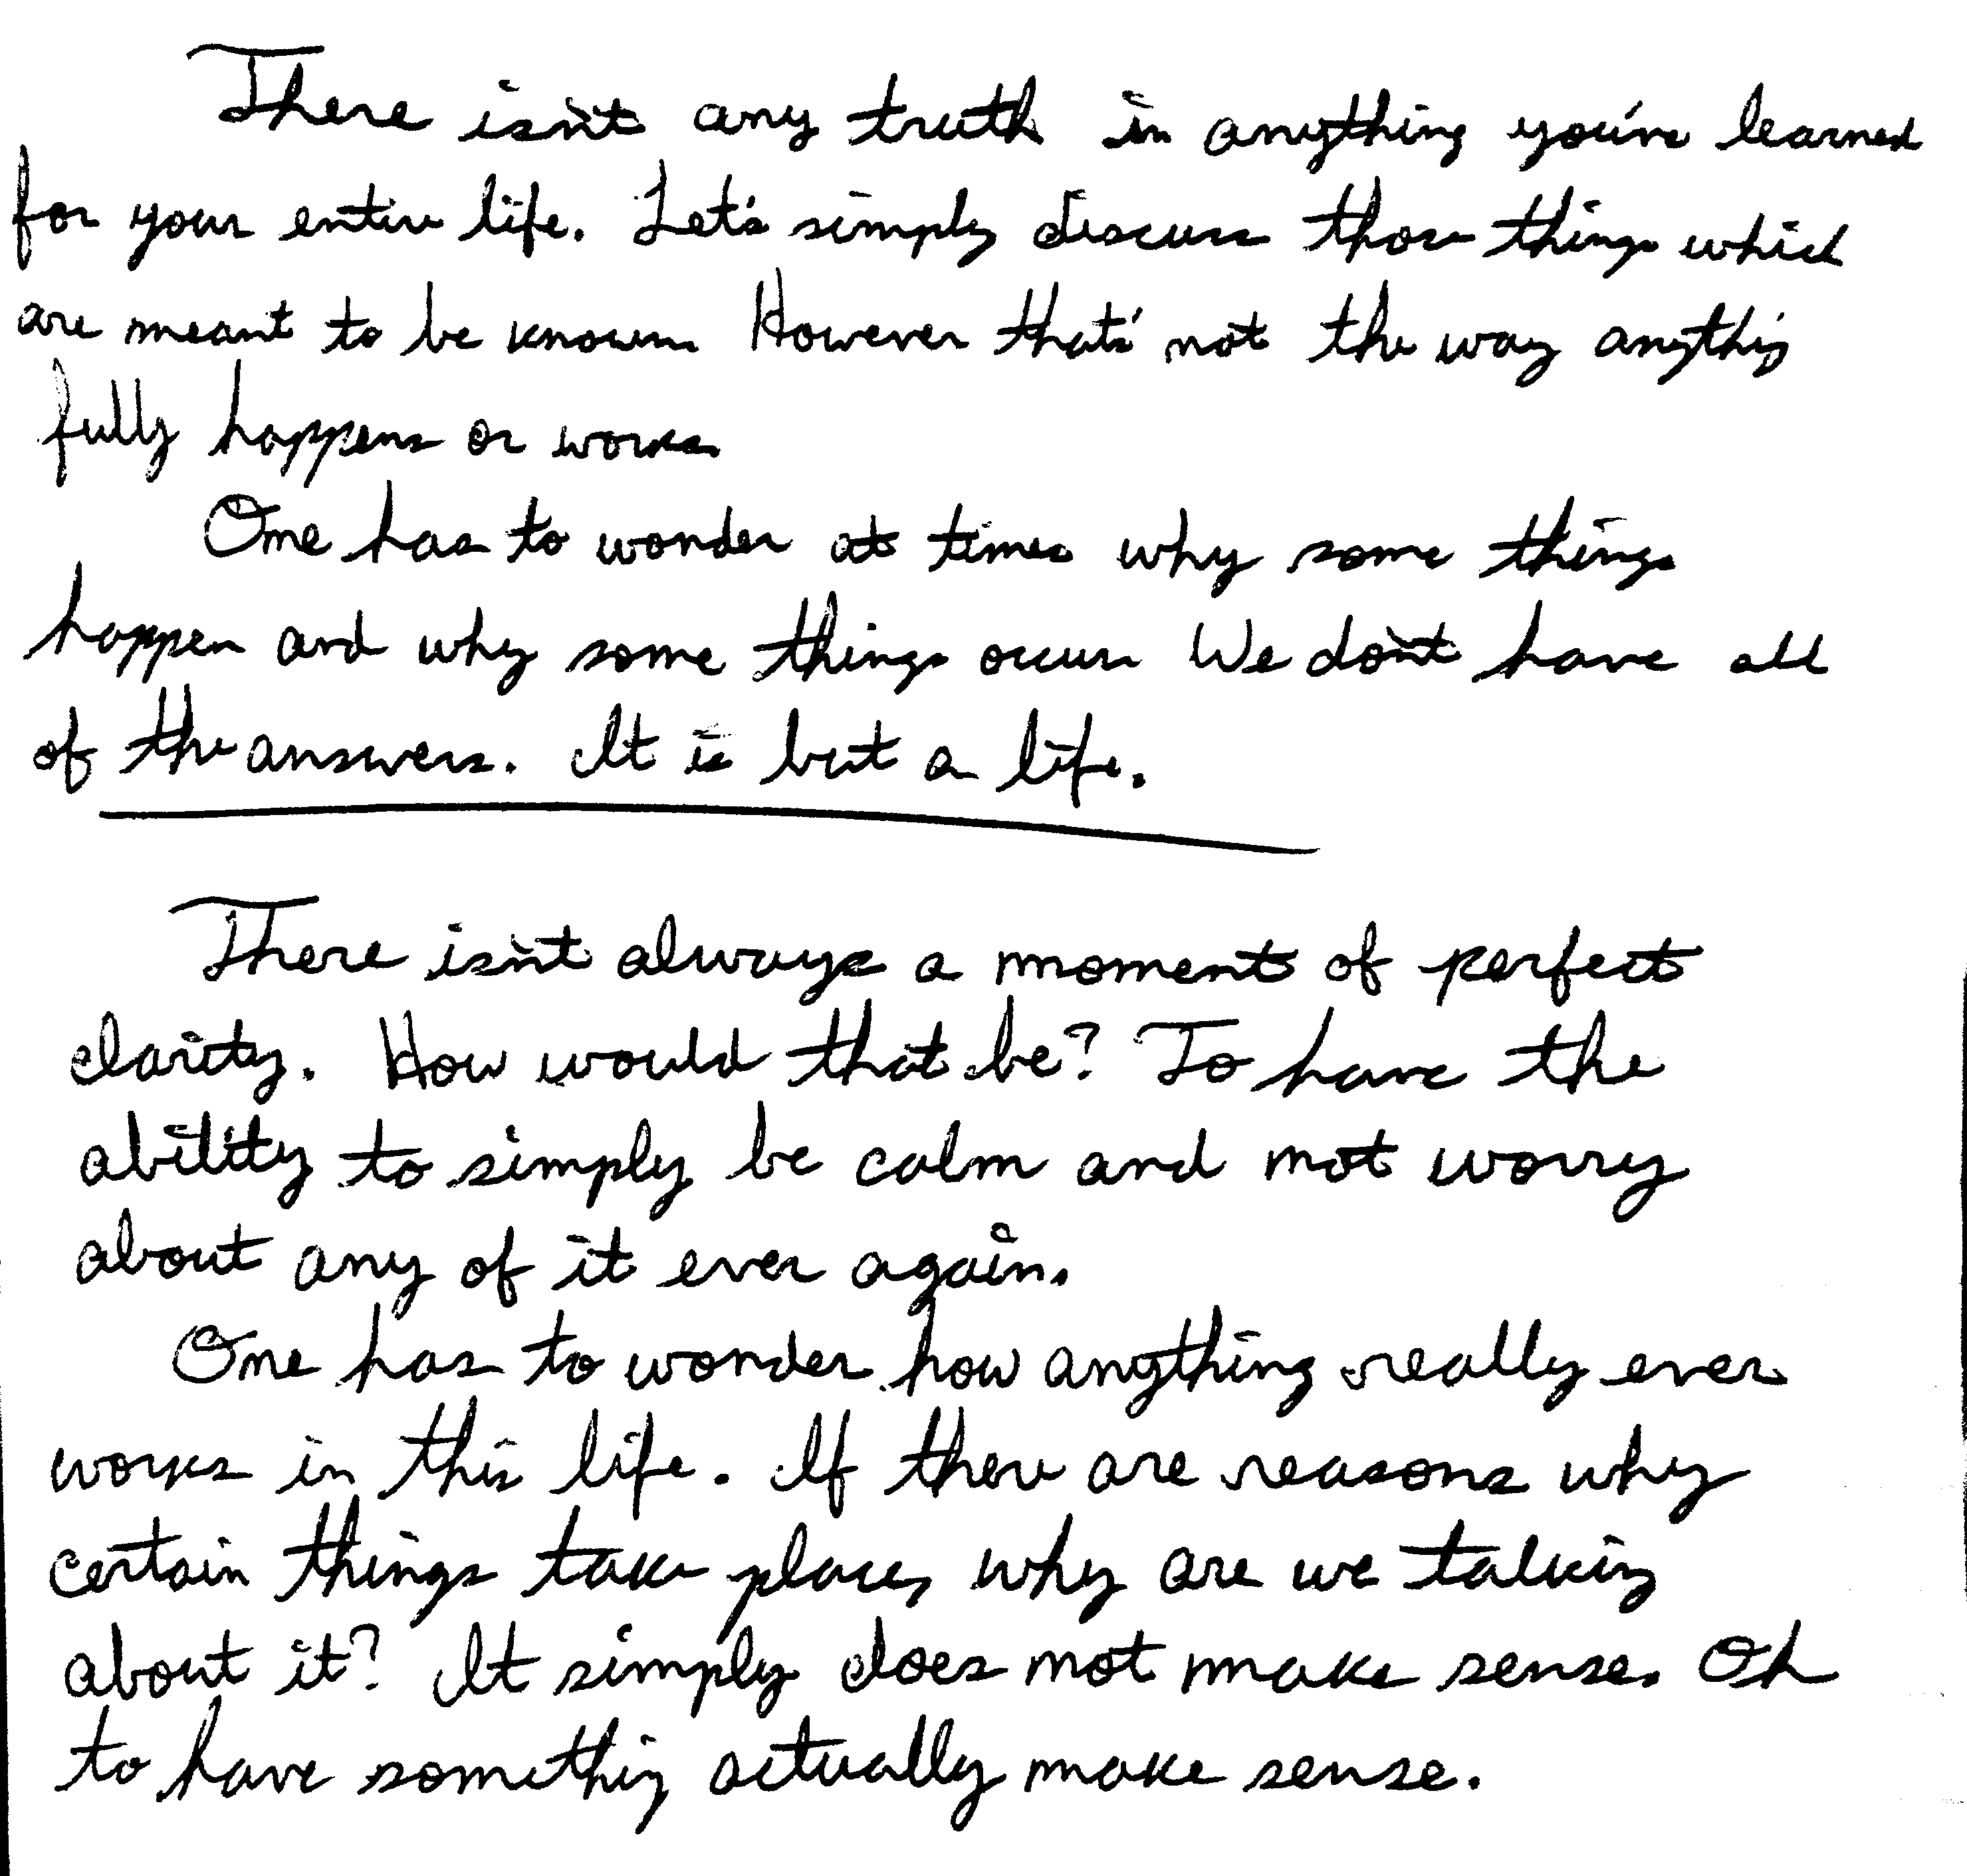
\includegraphics[width=.5\linewidth]{2018/images/handwriting.jpg}
  \caption{Handwriting}
  \label{fig:handwriting}
\end{figure}

Writing things down has a way of calming you. Be it handwriting, or electronically.
Either way? I feel handwriting has the ability to help out the most. When you can sit
down and write \st{some} experiences out on paper? It's a great feeling. It feels
right and has a way of calming you down. Talk about a breath of relief.

There comes a time in a person's life when all they want to do is sleep. They want to
forget everything about the rest of htis life and simply desire to fall asleep never
to wake up again. It is only a natural part of life is it not? Death is part of life.
There has never been any teachings contratry to that notion. It is the next
eveolutionary process in the steps of man.

So, why can't a person select the time of their own choosing? I mean, isn't it enough
to say ``hey, I'm done with this life. I'd like to go home now." Is that such a bad
thing? I do not know.

\begin{figure}[h!]
  \centering
  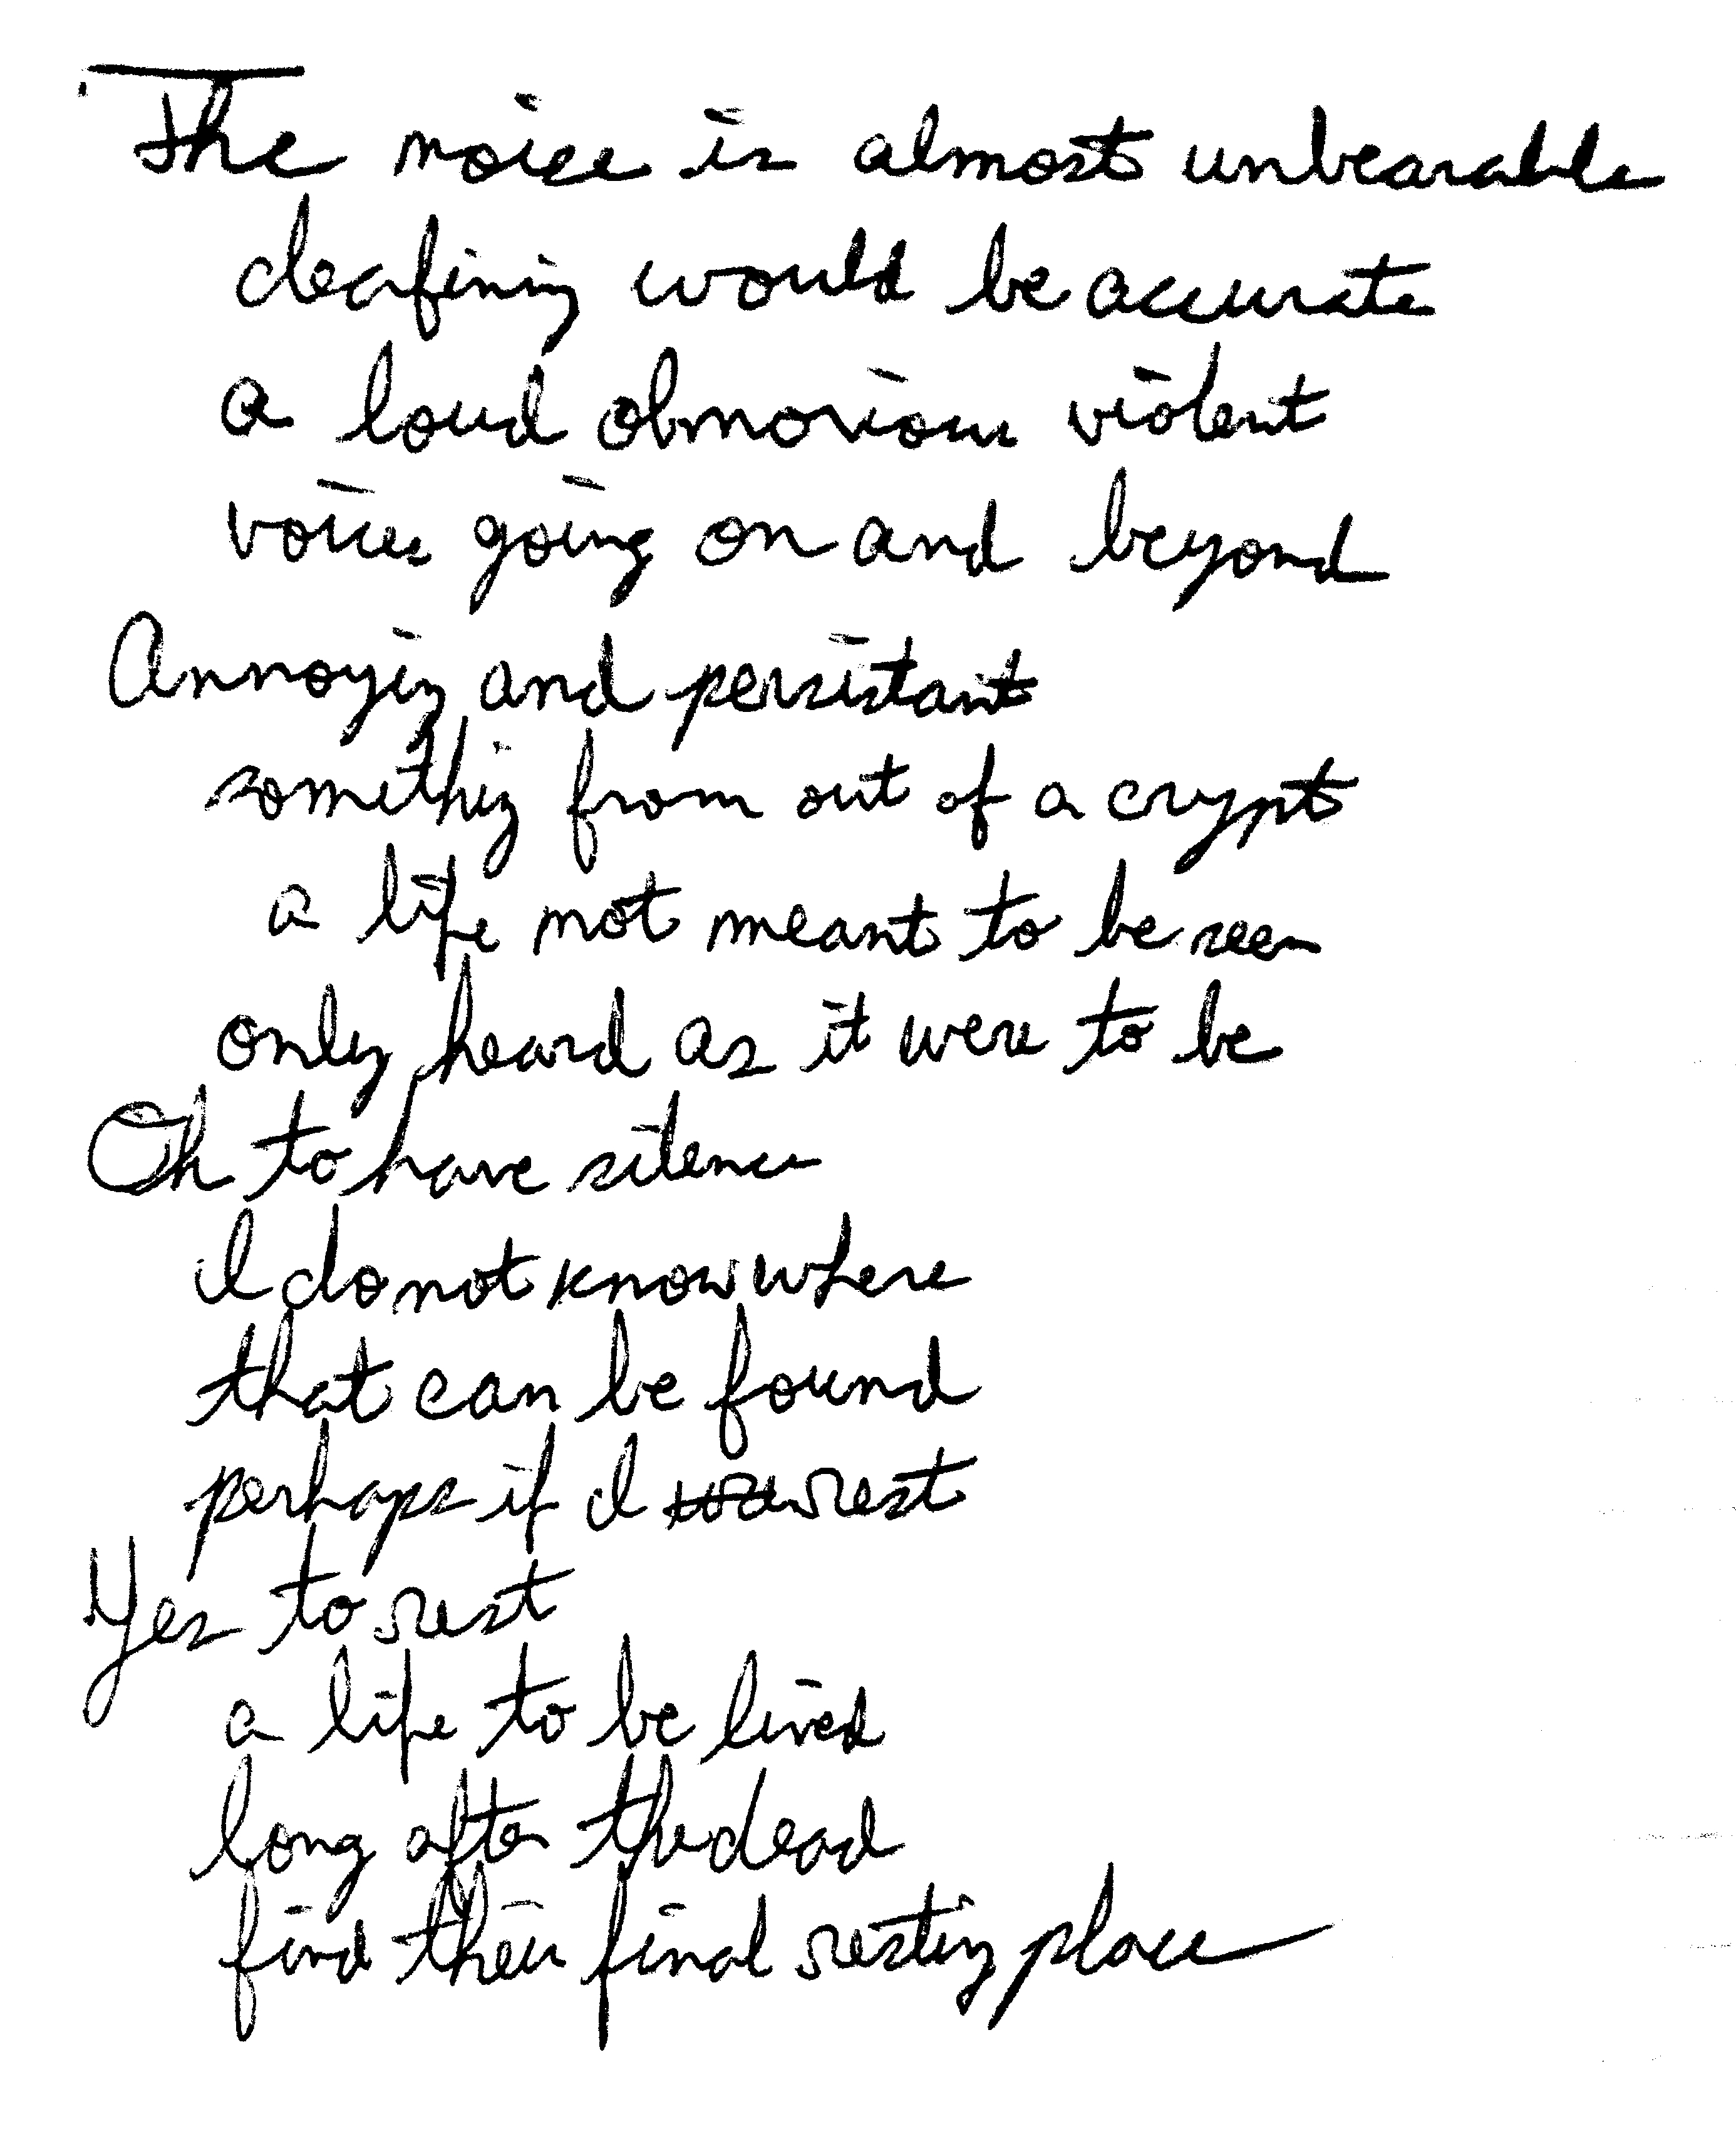
\includegraphics[width=.5\linewidth]{2018/images/rest.jpg}
  \caption{To Rest}
  \label{fig:rest}
\end{figure}

Perhaps it is a fixed point in time that we are unable to change. So many options and
changes come through this life, and here we are hoping one of them will be good
enough of a change for us ourselves. What if that's not the case at all? What if such
a change would have to come from a different source? We have agency, as it were, so
why cannot we enable such a change to be made and binding?

\section{Mon, Sep 24, 2018}

This week will feel like Hell.

Why do I feel this way? I'm not sure. I just have a feeling. Woke up with a panic
attack this morning. That's never a good sign for any week whatsoever. But I came
into work. Almost stayed home, but no I can't do that. A panic attack doesn't equate
to being sick. Anxiety runs in me. Fine. It's a fact. I cannot allow it to define who
I am.

\begin{figure}[h!]
  \centering
  \includegraphics[width=.5\linewidth]{2018/images/rabbit.jpg}
  \caption{Velveteen Rabbit}
  \label{fig:rabbit}
\end{figure}

``He said, `You become. It takes a long time. That's why it doesn't happen often to
people who break easily, or have sharp edges, or who have to be carefully kept.
Generally, by the time you are Real, most of your hair has been loved off, and your
eyes drop out and you get loose in the joints and very shabby. But these things don't
matter at all, because once you are Real you can't be ugly, except to people who
don't understand.'"\footnote{The Velveteen Rabbit}

Ah such a life to live. Not being ugly because you think you are not. To be able to
see past anything like that would be amazing. Not a lot of people grasp that concept,
unfortunately. There are so many things in this life we wish we could understand and
hold onto. Yet we don't. It's not an easy thing at all. It is but a life sure, but we
do not know why any of that happens to us. We are but living creatures.

\section{Mon, Apr 29, 2019}

There are so many questions that occur in this life. Why can't we always have the 
right answer to it all? Doesn't make sense does it? No, not really. Yet here
we are. We should find a way to simply understand something easier. Perhaps there
is another answer to this life. If there is? It should be an understanding. People
need to understand and be able to grasp what is to be understood. Does that make
any sense? I doubt it. It would be nice if it did have a way to make sense.

\chapter{June 2019}
\section{Fri, Oct 26, 2018}

Today is another Friday. It is a good thing I would suppose and hope for. I mean here
we are simply stating that the weekend is here. We can relax and enjoy that which we
are able to. It means nothing more than that. To be able to sit down and simply rest,
it is a good feeling.

There are some questions that come to mind at times. If that can be an accurate
statement. Sometimes those questions aren't easy to come by. Sometimes they aren't
easy to answer. Either way, we have questions. Questions which need to be answered.
Is that a bad thing? I'm not sure. It would be nice to be able to simply let it all
go by the wayside and just not worry about any of it.

Yet here I am. Wondering about things and how they end up being. Why are so many
things simply being in the way? Why must they have issues with life? It doesn't make
sense, it doesn't matter at times. Everything must be able to have peace. There must
be a way to find peace.\footnote{What exactly is peace though? People want peace all 
their days and they cannot find it. So, what causes peace to come down from whatever
place it is meant to come down? Doesn't make sense does it? No, I didn't think so.}



\chapter{Poetry}
\epigraph{All the world's a stage, And all the men and women merely players;}
{\textit{As You Like It \\ William Shakespeare}}
\section{Poem The First}

\poemtitle{We Don't Understand}
\settowidth{\versewidth}{Than Tycho Brahe, or Erra Pater:}
\begin{verse}
\poemlines{2}
It is but a day \\
to behold and the like \\
yet here we are \\
not understanding each other \\!

Here we are \\
staring across a room \\
a vast ocean as it were \\
and yet we don't know \\!

Who is to know \\
or understand \\
that which is meant \\
to be? \\!
\end{verse}
\attrib{Kyle Eggleston}
\section{Poem The Second}

\poemtitle{Why}
\settowidth{\versewidth}{Than Tycho Brahe, or Erra Pater:}
\begin{verse}
\poemlines{2}
Oh to ask that which is not \\
meant to be asked, why \\
but there is a time \\
when everything else \\
will find a path \\!
\end{verse}
\attrib{Kyle Eggleston (1979)}
\section{Poem The Third}

\poemtitle{Living Life}
\settowidth{\versewidth}{Than Tycho Brahe, or Erra Pater:}
\begin{verse}
\poemlines{2}
What is this life\\
upon which we live!\\
a meaningless chore\\
oh what a bore\\!

If I had a dream\\
to understand all\\
a place to grasp\\
maybe stand tall\\!

I'd go about\\
all of the land\\
the sea as it were\\
and preach of this life\\!

Yet here we are\\
learning afar\\
from heaven above\\
that romaing star\\!

We shouldn't grasp\\
for things not unseen\\
or fully misunderstood\\
but we sure can dream\\!
\end{verse}
\attrib{Kyle Eggleston (1979)}
\section{Poem The Fourth}

\poemtitle{To Be Human }
\settowidth{\versewidth}{Than Tycho Brahe, or Erra Pater:}
\begin{verse}
\poemlines{2}
Oh to be human\\
it is but a dream\\
wondering back and forth\\
on some light beam\\!

We do not understand\\
or fully can grasp\\
all that is happening\\
until the very last\\!

Some say this life\\
is but a curse\\
perhaps it would be better\\
if we had knowledge first\\!

So we hem and we haw\\
over land and the sea\\
wondering and waiting\\
oh what must this be?\\!

A life without end\\
or beginning it seems\\
we hope for a freedom\\
how brightly it gleams\\!

Waiting for a wonderful day\\
of bright sunshine and joy\\
don't be caught looking\\
down at a fake ploy\\!
\end{verse}
\attrib{Kyle Eggleston}

\backmatter
\printbibliography

\end{document}
